% =============================================================================
%  week15_diffusion.tex
%  Diffusion Models: From VAEs to DDPM — Full Mathematical Derivation
%  Morten Hjorth-Jensen, May 2026
%  Revised: code slides removed; VAE kept as motivation; new derivations added
% =============================================================================

\documentclass[aspectratio=169,11pt]{beamer}

\usetheme{Madrid}
\usecolortheme{default}
\usefonttheme[onlymath]{serif}

\setbeamercolor{frametitle}{bg=blue!11!white, fg=blue!60!white}
\setbeamercolor{title}{fg=blue!65!white}
\setbeamercolor{block title}{bg=blue!16!white, fg=blue!60!white}
\setbeamercolor{block body}{bg=blue!4!white}
\setbeamercolor{alerted text}{fg=red!65!black}
\setbeamertemplate{navigation symbols}{}
\setbeamertemplate{footline}{%
  \leavevmode\hbox{%
    \begin{beamercolorbox}[wd=.30\paperwidth,ht=2.25ex,dp=1ex,center]{author in head/foot}%
      \usebeamerfont{author in head/foot}\insertshortauthor
    \end{beamercolorbox}%
    \begin{beamercolorbox}[wd=.44\paperwidth,ht=2.25ex,dp=1ex,center]{title in head/foot}%
      \usebeamerfont{title in head/foot}\insertshorttitle
    \end{beamercolorbox}%
    \begin{beamercolorbox}[wd=.26\paperwidth,ht=2.25ex,dp=1ex,right]{date in head/foot}%
      \usebeamerfont{date in head/foot}\insertshortdate{}\hspace*{1em}%
      \insertframenumber/\inserttotalframenumber\hspace*{1ex}
    \end{beamercolorbox}}%
  \vskip0pt}

\usepackage[utf8]{inputenc}
\usepackage[T1]{fontenc}
\usepackage{amsmath,amssymb,amsfonts,mathtools,bm}
\usepackage{booktabs}
\usepackage{xcolor}
\usepackage{tikz}
\usetikzlibrary{arrows.meta,positioning,shapes.geometric,decorations.pathreplacing}
\usepackage{hyperref}

% ── Convenience macros ───────────────────────────────────────────────────────
\newcommand{\E}{\mathbb{E}}
\newcommand{\R}{\mathbb{R}}
\newcommand{\DKL}{D_{\mathrm{KL}}}
\newcommand{\Norm}{\mathcal{N}}
\newcommand{\ELBO}{\mathcal{L}}
\newcommand{\bx}{\bm{x}}
\newcommand{\bh}{\bm{h}}
\newcommand{\bz}{\bm{z}}
\newcommand{\beps}{\bm{\epsilon}}
\newcommand{\bmu}{\bm{\mu}}
\newcommand{\bsig}{\bm{\sigma}}
\newcommand{\btheta}{\bm{\theta}}
\newcommand{\bphi}{\bm{\phi}}
\newcommand{\half}{\tfrac{1}{2}}
% ── Additional macros for GAN section ────────────────────────────────────────
\newcommand{\pr}{p_{r}}           % real data distribution
\newcommand{\pg}{p_{g}}           % generator distribution
\newcommand{\pz}{p_{z}}           % noise prior
\newcommand{\JS}{D_{\mathrm{JS}}} % Jensen-Shannon divergence
\newcommand{\KL}{D_{\mathrm{KL}}} % alias matching GAN notation (= \DKL)
\DeclareMathOperator*{\argmax}{arg\,max}
\DeclareMathOperator*{\argmin}{arg\,min}

% ── Metadata ─────────────────────────────────────────────────────────────────
\title[Diffusion Models and GANs]{Denoising Diffusion Probabilistic Models and Generative Adversarial Networks}
\subtitle{From VAEs and Diffusion Models to GANs --- A Unified Derivation}
\author[M.\ Hjorth-Jensen]{Morten Hjorth-Jensen}
\institute[UiO/MSU]{Department of Physics \& CCSE, University of Oslo}
\date{May 4-8, 2026}

% =============================================================================
\begin{document}
% =============================================================================

\begin{frame}[plain]
  \titlepage
\end{frame}

% ── Table of contents ─────────────────────────────────────────────────────────
\begin{frame}[allowframebreaks]{Outline}
  \scriptsize
  \tableofcontents[hideallsubsections]
\end{frame}

% =============================================================================
\section{Motivation: VAEs and Their Limits}
% =============================================================================

% -----------------------------------------------------------------------------
\begin{frame}{Generative models: the common thread}

All deep generative models share one goal: learn a distribution
$p_{\btheta}(\bx)$ over data~$\bx$ that we can both evaluate and sample from.

\medskip
\begin{center}
\renewcommand{\arraystretch}{1.25}
\begin{tabular}{llll}
\toprule
\textbf{Family} & \textbf{Latent} & \textbf{Training signal} & \textbf{Sample cost}\\
\midrule
VAE            & $\bh \in \R^{d_h},\;d_h\!\ll\!d_x$ & ELBO             & 1 decoder pass\\
\textbf{Diffusion} & $\bx_t\in\R^{d_x}$ (full dim)  & \textbf{ELBO, $T$ levels} & $T$ denoiser calls\\
GAN            & $\bz\in\R^k$                       & Adversarial      & 1 generator pass\\
\bottomrule
\end{tabular}
\end{center}

\medskip
\begin{alertblock}{Key insight}
Diffusion models are \textbf{hierarchical VAEs} with $T$ latent levels,
a fixed (non-learned) encoder, and full-dimensional latents.
Understanding VAEs is the fastest route to understanding diffusion.
\end{alertblock}
\end{frame}

% -----------------------------------------------------------------------------
\begin{frame}{The VAE: ELBO and reparameterisation (recap)}

\textbf{Goal.} Maximise $\log p_{\btheta}(\bx)$ — intractable because
$p(\bx)=\int p_{\btheta}(\bx|\bh)\,p(\bh)\,d\bh$.

\medskip
Introduce approximate posterior $q_{\bphi}(\bh|\bx)$.
By Jensen's inequality on $\log$:
\[
  \log p(\bx)
  = \log\E_{q_{\bphi}(\bh|\bx)}\!\left[\frac{p_{\btheta}(\bx,\bh)}{q_{\bphi}(\bh|\bx)}\right]
  \;\geq\;
  \E_{q_{\bphi}(\bh|\bx)}\!\left[\log\frac{p_{\btheta}(\bx,\bh)}{q_{\bphi}(\bh|\bx)}\right]
  =: \ELBO(\bphi,\btheta).
\]
Splitting the joint $p(\bx,\bh)=p_{\btheta}(\bx|\bh)\,p(\bh)$:
\[
\boxed{
\ELBO(\bphi,\btheta)
= \underbrace{\E_{q_{\bphi}(\bh|\bx)}\!\left[\log p_{\btheta}(\bx|\bh)\right]}_{\text{reconstruction}}
- \underbrace{\DKL\!\bigl(q_{\bphi}(\bh|\bx)\,\|\,p(\bh)\bigr)}_{\text{regularisation}}}
\]

\textbf{Reparameterisation.}  With Gaussian encoder
$q_{\bphi}(\bh|\bx)=\Norm(\bmu_{\bphi},\bsig^2_{\bphi}\mathbf{I})$
and prior $p(\bh)=\Norm(\bm{0},\mathbf{I})$:
\[
  \bh = \bmu_{\bphi}(\bx) + \bsig_{\bphi}(\bx)\odot\beps,\quad
  \beps\sim\Norm(\bm{0},\mathbf{I}).
\]
Closed-form KL:
$\DKL(q\|p) = \frac{1}{2}\sum_{j}\!\left(\mu_j^2+\sigma_j^2-\log\sigma_j^2-1\right)$.
\end{frame}

% -----------------------------------------------------------------------------
\begin{frame}{Why VAEs produce blurry samples}

\textbf{The $\ell_2$-averaging problem.}
The decoder minimises
\[
  -\E_{q_{\bphi}}\!\left[\log p_{\btheta}(\bx|\bh)\right]
  \;\propto\;
  \E_{q_{\bphi}}\!\left[\|\bx - \hat{\bx}_{\btheta}(\bh)\|^2\right].
\]
Because the posterior $q_{\bphi}(\bh|\bx)$ has nonzero variance,
$\hat{\bx}_{\btheta}$ learns the \emph{mean over all likely completions},
which is systematically blurry.

\bigskip
\begin{columns}[T]
\column{0.5\textwidth}
\begin{block}{Other VAE limitations}
\begin{itemize}
  \item \textbf{Posterior collapse}: powerful decoder can ignore $\bh$,
        KL$\to 0$, latent useless.
  \item \textbf{ELBO gap}:
        $\log p(\bx) = \ELBO + \DKL(q_{\bphi}\|p(\bh|\bx)) > \ELBO$.
  \item Mean-field Gaussian approximation may miss
        multi-modal true posteriors.
\end{itemize}
\end{block}

\column{0.47\textwidth}
\begin{alertblock}{The diffusion solution}
\begin{itemize}
  \item Replace 1 latent level with $T\gg 1$.
  \item Fix the encoder: no collapse possible.
  \item Predict only the \emph{noise added at one step},
        not the full image — eliminates $\ell_2$-averaging artefacts.
\end{itemize}
\end{alertblock}
\end{columns}
\end{frame}

% =============================================================================
\section{Hierarchical VAEs and the Diffusion Limit}
% =============================================================================

% -----------------------------------------------------------------------------
\begin{frame}{Markovian hierarchical VAE (MHVAE)}

Generalise VAE to a \textbf{chain of $T$ latent spaces}
$\bx_1,\bx_2,\ldots,\bx_T$ (we already write $\bx_t$ for the $t$-th latent):

\begin{align*}
p(\bx_0,\bx_{1:T})
  &= p(\bx_T)\,p_{\btheta}(\bx_0|\bx_1)
     \prod_{t=2}^{T}p_{\btheta}(\bx_{t-1}|\bx_t)
     \quad\text{(generative)}\\[4pt]
q(\bx_{1:T}|\bx_0)
  &= q(\bx_1|\bx_0)
     \prod_{t=2}^{T}q(\bx_t|\bx_{t-1})
     \quad\text{(inference)}
\end{align*}

Substituting into the ELBO and using the Markov property:
\[
\log p(\bx_0)
\geq
\E_{q(\bx_{1:T}|\bx_0)}
\!\left[\log\frac{
    p(\bx_T)\,p_{\btheta}(\bx_0|\bx_1)
    \prod_{t=2}^{T}p_{\btheta}(\bx_{t-1}|\bx_t)}
  {q(\bx_1|\bx_0)\prod_{t=2}^{T}
    q(\bx_t|\bx_{t-1})}\right]
\]
Each level contributes a reconstruction/regularisation pair.
\end{frame}

% -----------------------------------------------------------------------------
\begin{frame}{Three constraints that define a diffusion model}

A \textbf{Variational Diffusion Model} (VDM; Kingma et al.\ 2021;
Luo 2022) is an MHVAE with three additional constraints:

\begin{block}{Constraint 1 — Full-dimensional latents}
$\dim(\bx_t) = \dim(\bx_0)$ for all $t$.
No bottleneck; the latents live in \emph{data space}.
\end{block}

\begin{block}{Constraint 2 — Fixed Gaussian encoder (forward process)}
\[
q(\bx_t|\bx_{t-1})
= \Norm\!\bigl(\bx_t;\,\sqrt{\alpha_t}\,\bx_{t-1},\,(1-\alpha_t)\mathbf{I}\bigr),
\quad \alpha_t = 1-\beta_t\in(0,1).
\]
Not trained. The noise schedule $\{\beta_t\}$ is a design choice.
\end{block}

\begin{block}{Constraint 3 — Gaussian terminal distribution}
$\{\alpha_t\}$ is chosen so that
$q(\bx_T|\bx_0)\approx\Norm(\bm{0},\mathbf{I})$
as $t\to T$.
The model ``forgets'' the data completely.
\end{block}
\end{frame}

% =============================================================================
\section{The Forward Process}
% =============================================================================

% -----------------------------------------------------------------------------
\begin{frame}{Forward process: the Gaussian product rule}

\textbf{Key tool.} If $\bx = a\bm{u} + b\bm{v}$ with
$\bm{u}\sim\Norm(\bm{0},\mathbf{I})$ and $\bm{v}\sim\Norm(\bm{0},\mathbf{I})$
independent, then
\[
  \bx \sim \Norm\!\bigl(\bm{0},\,(a^2+b^2)\mathbf{I}\bigr).
\]

\textbf{Proof of closed-form marginal.}
Write one step as $\bx_t = \sqrt{\alpha_t}\,\bx_{t-1} + \sqrt{1-\alpha_t}\,\beps_{t-1}$
with $\beps_{t-1}\sim\Norm(\bm{0},\mathbf{I})$.  Unrolling two steps:
\begin{align*}
\bx_t
&= \sqrt{\alpha_t}\bigl(\sqrt{\alpha_{t-1}}\,\bx_{t-2}
   + \sqrt{1-\alpha_{t-1}}\,\beps_{t-2}\bigr)
   + \sqrt{1-\alpha_t}\,\beps_{t-1}\\
&= \sqrt{\alpha_t\alpha_{t-1}}\,\bx_{t-2}
   + \underbrace{\sqrt{\alpha_t(1-\alpha_{t-1})}\,\beps_{t-2}
     + \sqrt{1-\alpha_t}\,\beps_{t-1}}_{\sim\,\Norm(\bm{0},\,
       [\alpha_t(1-\alpha_{t-1})+(1-\alpha_t)]\mathbf{I})}\\
&= \sqrt{\alpha_t\alpha_{t-1}}\,\bx_{t-2}
   + \sqrt{1-\alpha_t\alpha_{t-1}}\;\bar{\beps}
\end{align*}
since $\alpha_t(1-\alpha_{t-1})+(1-\alpha_t) = 1-\alpha_t\alpha_{t-1}$.
\end{frame}

% -----------------------------------------------------------------------------
\begin{frame}{Closed-form forward marginal $q(\bx_t|\bx_0)$}

Define $\bar\alpha_t = \prod_{s=1}^{t}\alpha_s$.  Continuing the induction:

\begin{block}{Closed-form marginal (key result)}
\[
\boxed{
  q(\bx_t|\bx_0)
  = \Norm\!\bigl(\bx_t;\;\sqrt{\bar\alpha_t}\,\bx_0,\;
    (1-\bar\alpha_t)\mathbf{I}\bigr)
}
\]
Equivalently, we can sample $\bx_t$ \emph{directly} in one step:
\[
  \bx_t = \sqrt{\bar\alpha_t}\,\bx_0 + \sqrt{1-\bar\alpha_t}\,\beps,
  \qquad \beps\sim\Norm(\bm{0},\mathbf{I}).
\]
\end{block}

\medskip
\textbf{Interpretation.}
\begin{itemize}
  \item $\sqrt{\bar\alpha_t}$ is the \emph{signal coefficient}: decays toward 0.
  \item $\sqrt{1-\bar\alpha_t}$ is the \emph{noise coefficient}: grows toward 1.
  \item At $t=0$: $\bx_0 = \bx_0$ (clean).
  \item At $t=T$: $\bx_T\approx\beps$ (pure noise).
\end{itemize}
No forward-pass through a network needed — this is just arithmetic.
\end{frame}

% -----------------------------------------------------------------------------
\begin{frame}{Signal-to-noise ratio and noise schedules}

Define the \textbf{signal-to-noise ratio}:
\[
  \mathrm{SNR}(t) = \frac{\bar\alpha_t}{1-\bar\alpha_t}.
\]
$\mathrm{SNR}(0)\gg 1$ (clean data); $\mathrm{SNR}(T)\approx 0$ (pure noise).
The VDM objective can be rewritten entirely in terms of $\mathrm{SNR}(t)$,
and the loss weight of each term equals $\mathrm{SNR}(t)-\mathrm{SNR}(t+1)$
(Kingma et al.\ 2021).

\bigskip
\begin{columns}[T]
\column{0.5\textwidth}
\textbf{Linear schedule} (Ho et al.\ 2020):
\[
  \beta_t = \beta_{\min} + \tfrac{t-1}{T-1}(\beta_{\max}-\beta_{\min})
\]
$\beta_{\min}=10^{-4}$, $\beta_{\max}=0.02$, $T=1000$.
\smallskip

Near-zero SNR early, then rapid collapse.

\column{0.48\textwidth}
\textbf{Cosine schedule} (Nichol \& Dhariwal 2021):
\[
  \bar\alpha_t = \frac{f(t)}{f(0)},\quad
  f(t) = \cos^2\!\!\left(\frac{t/T + s}{1+s}\cdot\frac{\pi}{2}\right)
\]
$s=0.008$. SNR decreases more gradually, improving training at low $t$.
\end{columns}

\medskip
The cosine schedule avoids the very small $\beta_t$ values that waste
early training steps on near-identical images.
\end{frame}

% =============================================================================
\section{The Forward Posterior}
% =============================================================================

% -----------------------------------------------------------------------------
\begin{frame}{Tractable forward posterior $q(\bx_{t-1}|\bx_t,\bx_0)$}

The \emph{unconditional} reverse $q(\bx_{t-1}|\bx_t)$ is intractable.
But conditioned on $\bx_0$ it is tractable via Bayes' rule:
\[
  q(\bx_{t-1}|\bx_t,\bx_0)
  = \frac{q(\bx_t|\bx_{t-1},\bx_0)\,q(\bx_{t-1}|\bx_0)}{q(\bx_t|\bx_0)}
  = \frac{q(\bx_t|\bx_{t-1})\,q(\bx_{t-1}|\bx_0)}{q(\bx_t|\bx_0)}.
\]
The last equality uses the Markov property: $q(\bx_t|\bx_{t-1},\bx_0)=q(\bx_t|\bx_{t-1})$.

\medskip
Each factor is Gaussian:
\begin{align*}
q(\bx_t|\bx_{t-1})    &= \Norm(\sqrt{\alpha_t}\,\bx_{t-1},\,(1-\alpha_t)\mathbf{I})\\
q(\bx_{t-1}|\bx_0)   &= \Norm(\sqrt{\bar\alpha_{t-1}}\,\bx_0,\,(1-\bar\alpha_{t-1})\mathbf{I})\\
q(\bx_t|\bx_0)        &= \Norm(\sqrt{\bar\alpha_t}\,\bx_0,\,(1-\bar\alpha_t)\mathbf{I})
\end{align*}
Substituting and completing the square in $\bx_{t-1}$
yields a Gaussian in $\bx_{t-1}$.
\end{frame}

% -----------------------------------------------------------------------------
\begin{frame}{Forward posterior: completing the square}

The log of the numerator (as a function of $\bx_{t-1}$) is:
\begin{align*}
&-\frac{(\bx_t - \sqrt{\alpha_t}\,\bx_{t-1})^2}{2(1-\alpha_t)}
 -\frac{(\bx_{t-1} - \sqrt{\bar\alpha_{t-1}}\,\bx_0)^2}{2(1-\bar\alpha_{t-1})}\\[4pt]
=\;&-\frac{1}{2}\left[
  \frac{\alpha_t}{1-\alpha_t}\bx_{t-1}^2
  - \frac{2\sqrt{\alpha_t}\,\bx_t}{1-\alpha_t}\bx_{t-1}
  + \frac{1}{1-\bar\alpha_{t-1}}\bx_{t-1}^2
  - \frac{2\sqrt{\bar\alpha_{t-1}}\,\bx_0}{1-\bar\alpha_{t-1}}\bx_{t-1}
  + \text{const}\right]
\end{align*}

Grouping the $\bx_{t-1}^2$ and $\bx_{t-1}$ terms gives a precision:
\[
  \frac{1}{\tilde\beta_t}
  = \frac{\alpha_t}{1-\alpha_t} + \frac{1}{1-\bar\alpha_{t-1}}
  = \frac{\alpha_t(1-\bar\alpha_{t-1}) + (1-\alpha_t)}{(1-\alpha_t)(1-\bar\alpha_{t-1})}
  = \frac{1-\bar\alpha_t}{(1-\alpha_t)(1-\bar\alpha_{t-1})}.
\]
Therefore:
\[
  \tilde\beta_t
  = \frac{(1-\alpha_t)(1-\bar\alpha_{t-1})}{1-\bar\alpha_t}
  = \frac{1-\bar\alpha_{t-1}}{1-\bar\alpha_t}\,\beta_t.
\]
\end{frame}

% -----------------------------------------------------------------------------
\begin{frame}{Forward posterior: the mean $\tilde{\bmu}_t$}

The mean of $q(\bx_{t-1}|\bx_t,\bx_0)$ is read off from the linear term:
\[
  \frac{\tilde{\bmu}_t}{\tilde\beta_t}
  = \frac{\sqrt{\alpha_t}\,\bx_t}{1-\alpha_t}
  + \frac{\sqrt{\bar\alpha_{t-1}}\,\bx_0}{1-\bar\alpha_{t-1}}.
\]
Multiplying through by $\tilde\beta_t$:
\begin{align*}
\tilde{\bmu}_t(\bx_t,\bx_0)
&= \frac{\sqrt{\alpha_t}(1-\bar\alpha_{t-1})}{1-\bar\alpha_t}\,\bx_t
 + \frac{\sqrt{\bar\alpha_{t-1}}\,\beta_t}{1-\bar\alpha_t}\,\bx_0
\end{align*}

\begin{block}{Forward posterior (exact result)}
\[
\boxed{
q(\bx_{t-1}|\bx_t,\bx_0)
= \Norm\!\bigl(\bx_{t-1};\;\tilde{\bmu}_t(\bx_t,\bx_0),\;\tilde\beta_t\mathbf{I}\bigr)
}
\]
\vspace{-2mm}
\[
\tilde{\bmu}_t(\bx_t,\bx_0)
= \frac{\sqrt{\alpha_t}(1-\bar\alpha_{t-1})}{1-\bar\alpha_t}\,\bx_t
+ \frac{\sqrt{\bar\alpha_{t-1}}\,\beta_t}{1-\bar\alpha_t}\,\bx_0,
\qquad
\tilde\beta_t = \frac{1-\bar\alpha_{t-1}}{1-\bar\alpha_t}\,\beta_t
\]
\end{block}

This is the \emph{target} the learned reverse process must match.
\end{frame}

% =============================================================================
\section{The ELBO and Its Decomposition}
% =============================================================================

% -----------------------------------------------------------------------------
\begin{frame}{VDM ELBO: full decomposition}
\small
Substituting the VDM structure into the MHVAE ELBO (Luo 2022, Sec.\ 3):

\vspace{-2pt}
\begin{align*}
\log p(\bx_0)
&\geq
\underbrace{\E_{q(\bx_1|\bx_0)}\!
  \bigl[\log p_{\btheta}(\bx_0|\bx_1)\bigr]}_{\mathcal{L}_0:\;\text{reconstruction}}
-\underbrace{\DKL\!\bigl(q(\bx_T|\bx_0)\|\,p(\bx_T)\bigr)}_{\mathcal{L}_T:\;\text{prior matching}}\\
&\quad
-\underbrace{\sum_{t=2}^{T}\E_{q(\bx_t|\bx_0)}\!
  \Bigl[\DKL\!\bigl(q(\bx_{t-1}|\bx_t,\bx_0)\|\,
               p_{\btheta}(\bx_{t-1}|\bx_t)\bigr)\Bigr]}_{\mathcal{L}_{1:T-1}:\;\text{denoising matching terms}}
\end{align*}

\vspace{-2pt}
\begin{itemize}
  \setlength\itemsep{2pt}
  \item $\mathcal{L}_T = 0$: schedule ensures $q(\bx_T|\bx_0)\approx\Norm(\bm{0},\mathbf{I})$.
  \item $\mathcal{L}_0$: single reconstruction step, treated separately.
  \item $\mathcal{L}_{1:T-1}$: dominant $T-1$ terms, each a Gaussian KL.
\end{itemize}
\end{frame}

% -----------------------------------------------------------------------------
\begin{frame}{Why condition on $\bx_0$ reduces variance}

\textbf{First attempt (naïve ELBO)} uses $q(\bx_{t-1}|\bx_t)$ in the KL,
which requires an expectation over \emph{two} random variables per term.
This has high Monte Carlo variance.

\medskip
\textbf{Second attempt (conditioned ELBO)} uses $q(\bx_{t-1}|\bx_t,\bx_0)$.
By the tower property:
\begin{align*}
  &\E_{q(\bx_{t-1},\bx_t|\bx_0)}\!\bigl[
    \DKL\!\bigl(q(\bx_{t-1}|\bx_t)\,\|\,p_{\btheta}(\bx_{t-1}|\bx_t)\bigr)\bigr]\\
  &\;\geq\;
  \E_{q(\bx_t|\bx_0)}\!\bigl[
    \DKL\!\bigl(q(\bx_{t-1}|\bx_t,\bx_0)\,\|\,p_{\btheta}(\bx_{t-1}|\bx_t)\bigr)\bigr].
\end{align*}
The conditioned form is a tighter bound \emph{and} requires sampling only
$\bx_t\sim q(\bx_t|\bx_0)$, which is one-shot via the closed-form marginal.
Each KL term now involves only a \textbf{single Monte Carlo draw}.

\begin{alertblock}{Practical consequence}
We compute $\bx_t = \sqrt{\bar\alpha_t}\,\bx_0 + \sqrt{1-\bar\alpha_t}\,\beps$
and evaluate the KL analytically — no expensive nested sampling.
\end{alertblock}
\end{frame}

% -----------------------------------------------------------------------------
\begin{frame}{Gaussian KL: closed-form evaluation}

Each denoising term is a KL between two Gaussians.
For general Gaussians $\mathcal{N}(\bmu_1,\Sigma_1)$ and
$\mathcal{N}(\bmu_2,\Sigma_2)$ in $\R^d$:
\[
  \DKL\!\bigl(\Norm(\bmu_1,\Sigma_1)\,\|\,\Norm(\bmu_2,\Sigma_2)\bigr)
  = \half\!\left[
    \log\frac{|\Sigma_2|}{|\Sigma_1|}
    - d
    + \mathrm{tr}(\Sigma_2^{-1}\Sigma_1)
    + (\bmu_2-\bmu_1)^\top\Sigma_2^{-1}(\bmu_2-\bmu_1)
  \right].
\]

\medskip
In our case both distributions have variance $\tilde\beta_t\mathbf{I}$,
so the $\log|\cdot|$ and $\mathrm{tr}(\cdot)$ terms cancel exactly:
\[
  \DKL\!\bigl(q(\bx_{t-1}|\bx_t,\bx_0)\,\|\,p_{\btheta}(\bx_{t-1}|\bx_t)\bigr)
  = \frac{1}{2\tilde\beta_t}
    \bigl\|\tilde{\bmu}_t(\bx_t,\bx_0) - \bmu_{\btheta}(\bx_t,t)\bigr\|^2
  + C
\]
where $p_{\btheta}(\bx_{t-1}|\bx_t)=\Norm(\bmu_{\btheta}(\bx_t,t),\tilde\beta_t\mathbf{I})$
and $C$ does not depend on $\btheta$.

\medskip
\textbf{Training reduces to matching means.}
The network only needs to predict $\tilde{\bmu}_t$.
\end{frame}

% =============================================================================
\section{Noise Prediction and the Training Objective}
% =============================================================================

% -----------------------------------------------------------------------------
\begin{frame}{Reparameterising $\tilde{\bmu}_t$ in terms of noise}

From the closed-form forward marginal:
$\bx_t = \sqrt{\bar\alpha_t}\,\bx_0 + \sqrt{1-\bar\alpha_t}\,\beps$,
we can solve for $\bx_0$:
\[
  \bx_0 = \frac{1}{\sqrt{\bar\alpha_t}}\bigl(\bx_t - \sqrt{1-\bar\alpha_t}\,\beps\bigr).
\]
Substituting into $\tilde{\bmu}_t(\bx_t,\bx_0)$:
\begin{align*}
\tilde{\bmu}_t(\bx_t,\beps)
&= \frac{\sqrt{\alpha_t}(1-\bar\alpha_{t-1})}{1-\bar\alpha_t}\,\bx_t
 + \frac{\sqrt{\bar\alpha_{t-1}}\,\beta_t}{1-\bar\alpha_t}
   \cdot\frac{\bx_t - \sqrt{1-\bar\alpha_t}\,\beps}{\sqrt{\bar\alpha_t}}\\
&= \frac{\sqrt{\alpha_t}(1-\bar\alpha_{t-1}) + \beta_t\sqrt{\bar\alpha_{t-1}/\bar\alpha_t}}{1-\bar\alpha_t}\,\bx_t
 - \frac{\beta_t\sqrt{\bar\alpha_{t-1}/\bar\alpha_t}\,\sqrt{1-\bar\alpha_t}}{1-\bar\alpha_t}\,\beps
\end{align*}

Using $\bar\alpha_t = \bar\alpha_{t-1}\alpha_t$ so $\sqrt{\bar\alpha_{t-1}/\bar\alpha_t}=1/\sqrt{\alpha_t}$,
and collecting terms (see next slide):
\end{frame}

% -----------------------------------------------------------------------------
\begin{frame}{The noise-parameterised mean}

After collecting terms in $\bx_t$ and $\beps$:
\[
  \tilde{\bmu}_t
  = \frac{1}{\sqrt{\alpha_t}}\!\left(
      \bx_t - \frac{\beta_t}{\sqrt{1-\bar\alpha_t}}\,\beps
    \right).
\]

\textbf{Verification.}
Numerator of $\bx_t$ coefficient:
$\alpha_t(1-\bar\alpha_{t-1}) + \beta_t/\alpha_t \cdot \bar\alpha_{t-1}/\bar\alpha_{t-1}$...
simplifies to $(1-\bar\alpha_t)/\sqrt{\alpha_t}$, giving coefficient $1/\sqrt{\alpha_t}$.\quad$\checkmark$

\medskip
If the network predicts noise
$\beps_{\btheta}(\bx_t,t)\approx\beps$, then choose:
\[
\bmu_{\btheta}(\bx_t,t)
= \frac{1}{\sqrt{\alpha_t}}\!\left(
    \bx_t - \frac{\beta_t}{\sqrt{1-\bar\alpha_t}}\,\beps_{\btheta}(\bx_t,t)
  \right).
\]

The denoising KL becomes:
\[
  \mathcal{L}_{t-1}
  = \E_{\bx_0,\beps}\!\left[
    \frac{\beta_t^2}{2\tilde\beta_t\,\alpha_t(1-\bar\alpha_t)}\,
    \bigl\|\beps - \beps_{\btheta}(\bx_t,t)\bigr\|^2
  \right]
\]
where $\bx_t = \sqrt{\bar\alpha_t}\,\bx_0 + \sqrt{1-\bar\alpha_t}\,\beps$.
\end{frame}

% -----------------------------------------------------------------------------
\begin{frame}{The simplified DDPM training objective}

Ho et al.\ (2020) observed empirically that \textbf{dropping the time-dependent
weighting} $\beta_t^2/(2\tilde\beta_t\alpha_t(1-\bar\alpha_t))$ and averaging
uniformly over $t$ gives a simpler objective with \emph{better} sample quality:

\begin{block}{DDPM training loss $\mathcal{L}_{\mathrm{simple}}$}
\[
\boxed{
\mathcal{L}_{\mathrm{simple}}
= \E_{t\sim\mathrm{U}[1,T],\;\bx_0,\;\beps\sim\Norm(\bm{0},\mathbf{I})}\!\left[
  \bigl\|\beps
         - \beps_{\btheta}\!\left(
             \sqrt{\bar\alpha_t}\,\bx_0
             + \sqrt{1-\bar\alpha_t}\,\beps,\;t
           \right)\bigr\|^2
\right]
}
\]
\end{block}

\medskip
\textbf{Intuition.}
Dropping the weight up-weights early steps (small $t$, small noise, easy
to denoise) relative to later steps. This has a regularising effect:
the network focuses more on the hard tasks where its predictions matter.
The original weighted sum is still a valid ELBO; the simple loss is a
reweighted ELBO that happens to work better in practice.
\end{frame}

% -----------------------------------------------------------------------------
\begin{frame}{Three equivalent parameterisations}
\small
$\bx_t,\bx_0,\beps$ satisfy a linear equation, so predicting any one is equivalent:

\vspace{3pt}
\begin{center}
\renewcommand{\arraystretch}{1.2}
\begin{tabular}{llp{4.4cm}}
\toprule
\textbf{Predict} & \textbf{Objective} & \textbf{Notes}\\
\midrule
$\beps$ (noise) &
  $\|\beps - \beps_{\btheta}(\bx_t,t)\|^2$ &
  DDPM; most common\\[3pt]
$\bx_0$ (data) &
  $\|\bx_0 - \hat\bx_{\btheta}(\bx_t,t)\|^2$ &
  Can over-smooth\\[3pt]
$\bm{v} = \sqrt{\bar\alpha_t}\beps - \sqrt{1-\bar\alpha_t}\bx_0$ &
  $\|\bm{v} - \bm{v}_{\btheta}(\bx_t,t)\|^2$ &
  Velocity; stable at $t\!\to\!0$\\
\bottomrule
\end{tabular}
\end{center}

\vspace{4pt}
\textbf{Conversions at inference:}
\[
\hat\bx_0 = \frac{\bx_t - \sqrt{1-\bar\alpha_t}\,\beps_{\btheta}}{\sqrt{\bar\alpha_t}},
\qquad
\hat\beps = \frac{\bx_t - \sqrt{\bar\alpha_t}\,\hat\bx_0}{\sqrt{1-\bar\alpha_t}}.
\]
All three targets give the same denoising KL when substituted back.
\end{frame}

% =============================================================================
\section{Connection to Score Matching}
% =============================================================================

% -----------------------------------------------------------------------------
\begin{frame}{The score function}

The \textbf{score} of a distribution $p(\bx)$ is
$\nabla_{\bx}\log p(\bx)$.
It points towards regions of high probability density.

\medskip
\textbf{Score of the forward-diffused distribution.}
Since
$q(\bx_t|\bx_0) = \Norm(\sqrt{\bar\alpha_t}\,\bx_0,(1-\bar\alpha_t)\mathbf{I})$,
its log-density is:
\[
  \log q(\bx_t|\bx_0)
  = -\frac{1}{2(1-\bar\alpha_t)}\|\bx_t - \sqrt{\bar\alpha_t}\,\bx_0\|^2 + C.
\]
Differentiating with respect to $\bx_t$:
\[
  \nabla_{\bx_t}\log q(\bx_t|\bx_0)
  = -\frac{\bx_t - \sqrt{\bar\alpha_t}\,\bx_0}{1-\bar\alpha_t}
  = -\frac{\beps}{\sqrt{1-\bar\alpha_t}}.
\]
The score is proportional to the \emph{negative noise}.
\end{frame}

% -----------------------------------------------------------------------------
\begin{frame}{DDPM as denoising score matching}

Define the learned score network $\bm{s}_{\btheta}(\bx_t,t)$.
The \textbf{score matching objective} minimises:
\[
  \E_{t,\bx_t}\!\left[\bigl\|\nabla_{\bx_t}\log q(\bx_t) - \bm{s}_{\btheta}(\bx_t,t)\bigr\|^2\right].
\]

The \textbf{denoising score matching} (Vincent 2011) substitution:
\[
  \nabla_{\bx_t}\log q(\bx_t)
  = \E_{q(\bx_0|\bx_t)}\!\left[\nabla_{\bx_t}\log q(\bx_t|\bx_0)\right]
  = -\E_{q(\bx_0|\bx_t)}\!\left[\frac{\beps}{\sqrt{1-\bar\alpha_t}}\right].
\]

With the optimal score network $\bm{s}^*_{\btheta}(\bx_t,t)=-\beps^*/\sqrt{1-\bar\alpha_t}$:
\[
  \bm{s}_{\btheta}(\bx_t,t)
  = -\frac{\beps_{\btheta}(\bx_t,t)}{\sqrt{1-\bar\alpha_t}}
  \;\;\Longrightarrow\;\;
  \bm{s}^*_{\btheta}\approx\nabla_{\bx_t}\log q(\bx_t).
\]

\begin{alertblock}{Equivalence}
\textbf{DDPM noise prediction = denoising score matching.}
The DDPM network implicitly learns the score of the noisy data distribution
at every noise level simultaneously.
\end{alertblock}
\end{frame}

% -----------------------------------------------------------------------------
\begin{frame}{From score to SDE: the continuous-time limit}

Song et al.\ (2021) embed the discrete chain into a continuous SDE.
As $T\to\infty$ with $\beta_t\to\beta(t)\,dt$, the forward process becomes:
\[
  d\bx = -\tfrac{1}{2}\beta(t)\,\bx\,dt + \sqrt{\beta(t)}\,d\bm{W}_t,
\]
where $\bm{W}_t$ is Brownian motion.  By Anderson (1982), the
\textbf{reverse SDE} is:
\[
  d\bx = \bigl[-\tfrac{1}{2}\beta(t)\,\bx
               - \beta(t)\,\nabla_{\bx}\log p_t(\bx)\bigr]\,dt
         + \sqrt{\beta(t)}\,d\bar{\bm{W}}_t
\]
where $\bar{\bm{W}}_t$ is reverse-time Brownian motion.
Replacing the score by the learned network gives:
\[
d\bx = \bigl[-\tfrac{1}{2}\beta(t)\,\bx
             + \beta(t)\,\tfrac{\beps_{\btheta}(\bx,t)}{\sqrt{1-\bar\alpha_t}}\bigr]\,dt
       + \sqrt{\beta(t)}\,d\bar{\bm{W}}_t.
\]
The same network $\beps_{\btheta}$ that DDPM trains is the score estimator
that drives the reverse SDE.
\end{frame}

% =============================================================================
\section{The Reverse Process and Sampling}
% =============================================================================

% -----------------------------------------------------------------------------
\begin{frame}{The learned reverse process}

Choose the learned reverse as:
\[
  p_{\btheta}(\bx_{t-1}|\bx_t)
  = \Norm\!\bigl(\bx_{t-1};\;\bmu_{\btheta}(\bx_t,t),\;\tilde\beta_t\mathbf{I}\bigr)
\]
with $\bmu_{\btheta}$ the noise-parameterised mean from Section~4.

\medskip
\textbf{Why use $\tilde\beta_t$ as the reverse variance?}
The true posterior variance $\tilde\beta_t$ lies between
$\beta_t$ (upper bound, for $q(\bx_{t-1}|\bx_t)$) and
$\tilde\beta_t$ (exact, for $q(\bx_{t-1}|\bx_t,\bx_0)$).
Ho et al.\ fixed it to $\tilde\beta_t$; later work (Nichol \& Dhariwal 2021)
learns it as an interpolation:
\[
  \Sigma_{\btheta}(\bx_t,t)
  = \exp\bigl(v\log\beta_t + (1-v)\log\tilde\beta_t\bigr),
  \quad v = v_{\btheta}(\bx_t,t)\in[0,1].
\]

\begin{block}{DDPM reverse step}
\[
  \bx_{t-1} = \frac{1}{\sqrt{\alpha_t}}\!\left(
    \bx_t - \frac{\beta_t}{\sqrt{1-\bar\alpha_t}}\,\beps_{\btheta}(\bx_t,t)
  \right)
  + \sqrt{\tilde\beta_t}\,\bz,\quad
  \bz\sim\Norm(\bm{0},\mathbf{I})\;(t>1),\;\bz=\bm{0}\;(t=1).
\]
\end{block}
\end{frame}

% -----------------------------------------------------------------------------
\begin{frame}{DDPM reverse algorithm}

\begin{block}{Complete DDPM sampling procedure}
\begin{enumerate}
  \setlength\itemsep{5pt}
  \item Sample $\bx_T\sim\Norm(\bm{0},\mathbf{I})$.
  \item For $t = T,\, T-1,\,\ldots,\,1$:
    \begin{enumerate}
      \item $\bz\sim\Norm(\bm{0},\mathbf{I})$ if $t>1$;\quad $\bz=\bm{0}$ if $t=1$.
      \item Predict noise: $\hat\beps = \beps_{\btheta}(\bx_t,t)$.
      \item Update:
        $\displaystyle\bx_{t-1}
         = \frac{1}{\sqrt{\alpha_t}}\!\left(
             \bx_t - \frac{\beta_t}{\sqrt{1-\bar\alpha_t}}\,\hat\beps
           \right)
           + \sqrt{\tilde\beta_t}\,\bz$.
    \end{enumerate}
  \item Return $\bx_0$.
\end{enumerate}
\end{block}

\medskip
\begin{itemize}
  \item Each step is one network evaluation plus a cheap Gaussian update.
  \item With $T=1000$: slow but high quality.
  \item \textbf{No discriminator}, no adversarial dynamics, no mode collapse.
\end{itemize}
\end{frame}

% =============================================================================
\section{Faster Sampling: DDIM}
% =============================================================================

% -----------------------------------------------------------------------------
\begin{frame}{DDIM: deterministic ODE sampling}
\small
The DDPM score network is \emph{independent of the sampling procedure},
so the stochastic SDE can be replaced by a deterministic ODE:
\[
  d\bx = \Bigl[\tfrac{\bx - \sqrt{1-\bar\alpha}\,\beps_{\btheta}(\bx,\bar\alpha)}
               {\sqrt{\bar\alpha}}\Bigr]\, d\sqrt{\bar\alpha}.
\]
Discretise over a subsequence $\tau_1<\cdots<\tau_S$ ($S\ll T$):
\begin{block}{DDIM update ($\sigma_{\tau_i}=\eta\sqrt{\tilde\beta_{\tau_i}}$)}
\vspace{-4pt}
\[
  \bx_{\tau_{i-1}}
  = \sqrt{\bar\alpha_{\tau_{i-1}}}\,\hat\bx_0
  + \sqrt{1-\bar\alpha_{\tau_{i-1}} - \sigma_{\tau_i}^2}\;\beps_{\btheta}(\bx_{\tau_i},\tau_i)
  + \sigma_{\tau_i}\bz,
\]
\vspace{-6pt}
\[
  \hat\bx_0 = \tfrac{\bx_{\tau_i}-\sqrt{1-\bar\alpha_{\tau_i}}\,\beps_{\btheta}(\bx_{\tau_i},\tau_i)}
                    {\sqrt{\bar\alpha_{\tau_i}}}.
\]
\end{block}
\vspace{-2pt}
\begin{itemize}
  \setlength\itemsep{2pt}
  \item $\eta=0$: fully deterministic — same $\bx_T$ always gives same $\bx_0$.
  \item $\eta=1$: recovers DDPM stochastic sampling.
  \item $S=50$ matches quality of $T=1000$ DDPM steps.
\end{itemize}
\end{frame}

% -----------------------------------------------------------------------------
\begin{frame}{DDIM: derivation of the update rule}

Start from the DDIM non-Markovian inference distribution (Song et al.\ 2020):
\[
  q_\sigma(\bx_{\tau_{i-1}}|\bx_{\tau_i},\bx_0)
  = \Norm\!\bigl(\bx_{\tau_{i-1}};\;
    \sqrt{\bar\alpha_{\tau_{i-1}}}\,\bx_0
    + \sqrt{1-\bar\alpha_{\tau_{i-1}}-\sigma^2}\;\tfrac{\bx_{\tau_i}-\sqrt{\bar\alpha_{\tau_i}}\,\bx_0}{\sqrt{1-\bar\alpha_{\tau_i}}},\;
    \sigma^2\mathbf{I}\bigr).
\]

Replacing $\bx_0$ by the predicted $\hat\bx_0$ and the exact noise direction
by $\beps_{\btheta}(\bx_{\tau_i},\tau_i)$ recovers the update rule on the
previous slide.

\medskip
\textbf{Why does this work?}
The DDIM update is a first-order ODE solver for the probability-flow ODE.
The ODE and the reverse SDE share the same marginals
$p_t(\bx_t)$ at every time $t$.
Since $\beps_{\btheta}$ approximates the score of $p_t$,
integrating the ODE gives the same distribution over $\bx_0$
as ancestral sampling from the reverse SDE — but in far fewer steps.
\end{frame}

% =============================================================================
\section{Latent Diffusion and Connections}
% =============================================================================

% -----------------------------------------------------------------------------
\begin{frame}{Latent Diffusion Models (Stable Diffusion)}

\textbf{Problem.} DDPM in pixel space ($512\!\times\!512\!\times\!3=786\,432$ dims) is too expensive.

\smallskip
\textbf{Solution} (Rombach et al.\ 2022): run diffusion in a compressed VAE latent space.

\begin{enumerate}
  \setlength\itemsep{2pt}
  \item \textbf{VAE encoder}: $\bx\in\R^{H\times W\times 3}
        \to\bz\in\R^{H/8\times W/8\times 4}$ ($\approx\!48\times$ compression).
  \item \textbf{DDPM in} $\bz$: much cheaper than pixel space.
  \item \textbf{VAE decoder}: $\hat\bz_0\to\hat\bx$.
\end{enumerate}

\begin{block}{Why this works}
\begin{itemize}
  \setlength\itemsep{1pt}
  \item VAE latent is perceptually smooth and semantically structured.
  \item Diffusion on $\bz$ skips low-level pixel correlations.
  \item Conditioning (text, depth, class) via cross-attention in the U-Net.
  \item KL regularisation keeps $\bz$ smooth enough for the diffusion prior.
\end{itemize}
\end{block}
\end{frame}

% -----------------------------------------------------------------------------
\begin{frame}{VAE vs.\ Diffusion: mathematical parallel}
\small
Both maximise $\log p(\bx)\geq\ELBO(\bphi,\btheta)
=\E[\log p_{\btheta}(\bx|\bz)]-\DKL(q_{\bphi}\|p)$.
Differences lie in how this framework is applied:

\begin{center}
\renewcommand{\arraystretch}{1.15}
\begin{tabular}{lll}
\toprule
\textbf{Design axis} & \textbf{VAE} & \textbf{DDPM}\\
\midrule
Latent levels    & 1                    & $T = 300$--$1000$\\
Encoder          & Learned $q_{\bphi}$  & Fixed schedule\\
Bottleneck       & Yes ($d_h\ll d_x$)   & No ($d_h = d_x$)\\
Network predicts & $\bx$ from $\bh$     & $\beps$ from $(\bx_t,t)$\\
KL terms         & 1                    & $T-1$\\
Training loss    & BCE $+$ $\DKL$       & MSE (noise)\\
Sampling cost    & 1 decoder call       & $T$ denoiser calls\\
\bottomrule
\end{tabular}
\end{center}

\begin{block}{Key insight}
DDPM $=$ VAE with (a) $T$ latent levels, (b) fixed encoder, (c) no bottleneck.
\end{block}
\end{frame}

% -----------------------------------------------------------------------------
\begin{frame}{VAE vs.\ Diffusion: pros and cons}

\begin{columns}[T]
\column{0.5\textwidth}
\begin{block}{VAE}
\textcolor{green!60!black}{\textbf{Pros:}}
\begin{itemize}\footnotesize\setlength\itemsep{1pt}
  \item Fast inference (1 pass)
  \item Compact structured latent space
  \item Stable training, closed-form KL
  \item Good for clustering / interpolation
  \item Scalable to large datasets
\end{itemize}
\textcolor{red!60!black}{\textbf{Cons:}}
\begin{itemize}\footnotesize\setlength\itemsep{1pt}
  \item \textbf{Blurry samples} ($\ell_2$-averaging)
  \item Posterior collapse risk
  \item ELBO gap (log-likelihood not exact)
  \item Mean-field limits posterior quality
\end{itemize}
\end{block}

\column{0.5\textwidth}
\begin{block}{Diffusion (DDPM)}
\textcolor{green!60!black}{\textbf{Pros:}}
\begin{itemize}\footnotesize\setlength\itemsep{1pt}
  \item \textbf{State-of-the-art} sample quality
  \item No mode collapse
  \item Stable training (MSE, no adversary)
  \item Grounded via ELBO + score matching
  \item Flexible conditioning
\end{itemize}
\textcolor{red!60!black}{\textbf{Cons:}}
\begin{itemize}\footnotesize\setlength\itemsep{1pt}
  \item \textbf{Slow} sampling ($T$ evaluations)
  \item No compact latent space
  \item High memory for large $T$
  \item Less natural for representation learning
\end{itemize}
\end{block}
\end{columns}
\end{frame}

% =============================================================================
\section{Summary and Exercises}
% =============================================================================

% -----------------------------------------------------------------------------
\begin{frame}{Key equations: complete reference}

\begin{center}\small
\renewcommand{\arraystretch}{1.4}
\begin{tabular}{ll}
\toprule
\textbf{Concept} & \textbf{Formula}\\
\midrule
Forward step &
  $q(\bx_t|\bx_{t-1}) = \Norm(\sqrt{\alpha_t}\,\bx_{t-1},\,(1-\alpha_t)\mathbf{I})$\\
Forward marginal &
  $q(\bx_t|\bx_0) = \Norm(\sqrt{\bar\alpha_t}\,\bx_0,\,(1-\bar\alpha_t)\mathbf{I})$\\
One-shot sample &
  $\bx_t = \sqrt{\bar\alpha_t}\,\bx_0 + \sqrt{1-\bar\alpha_t}\,\beps$\\
Forward posterior mean &
  $\tilde\bmu_t = \frac{\sqrt{\alpha_t}(1-\bar\alpha_{t-1})}{1-\bar\alpha_t}\bx_t
    + \frac{\sqrt{\bar\alpha_{t-1}}\beta_t}{1-\bar\alpha_t}\bx_0$\\
Forward posterior var. &
  $\tilde\beta_t = \frac{1-\bar\alpha_{t-1}}{1-\bar\alpha_t}\,\beta_t$\\
Noise-param.\ mean &
  $\tilde\bmu_t = \frac{1}{\sqrt{\alpha_t}}\!\bigl(\bx_t - \frac{\beta_t}{\sqrt{1-\bar\alpha_t}}\beps\bigr)$\\
Training loss &
  $\mathcal{L}_{\mathrm{simple}} = \E\bigl[\|\beps - \beps_{\btheta}(\bx_t,t)\|^2\bigr]$\\
Score relation &
  $\bm{s}_{\btheta}(\bx_t,t) = -\beps_{\btheta}(\bx_t,t)/\sqrt{1-\bar\alpha_t}$\\
Reverse step &
  $\bx_{t-1} = \frac{1}{\sqrt{\alpha_t}}\!\bigl(\bx_t - \frac{\beta_t}{\sqrt{1-\bar\alpha_t}}\beps_{\btheta}\bigr) + \sqrt{\tilde\beta_t}\,\bz$\\
SNR &
  $\mathrm{SNR}(t) = \bar\alpha_t/(1-\bar\alpha_t)$\\
\bottomrule
\end{tabular}
\end{center}
\end{frame}

% -----------------------------------------------------------------------------
\begin{frame}{Exercises}
\begin{columns}[T]
\column{0.5\textwidth}
\begin{block}{Exercises 1--3}
\footnotesize
\begin{enumerate}
  \setlength\itemsep{4pt}
  \item \textbf{Forward marginal.}
        Prove $q(\bx_t|\bx_0)=\Norm(\sqrt{\bar\alpha_t}\bx_0,(1-\bar\alpha_t)\mathbf{I})$
        by induction from $q(\bx_t|\bx_{t-1})$.

  \item \textbf{Forward posterior.}
        Apply Bayes' rule to derive $q(\bx_{t-1}|\bx_t,\bx_0)$.
        Show that completing the square gives $\tilde\bmu_t$ and $\tilde\beta_t$.

  \item \textbf{Gaussian KL.}
        Derive $\DKL(\Norm(\bmu_1,\sigma^2\mathbf{I})\|\Norm(\bmu_2,\sigma^2\mathbf{I}))
        = \|\bmu_1-\bmu_2\|^2/(2\sigma^2)$ and verify
        that the trace and log-det terms cancel exactly.
\end{enumerate}
\end{block}

\column{0.5\textwidth}
\begin{block}{Exercises 4--6}
\footnotesize
\begin{enumerate}
  \setlength\itemsep{4pt}
  \setcounter{enumi}{3}
  \item \textbf{Noise reparameterisation.}
        Substitute $\bx_0=(\bx_t-\sqrt{1-\bar\alpha_t}\beps)/\sqrt{\bar\alpha_t}$
        into $\tilde\bmu_t$ and verify the result equals
        $\frac{1}{\sqrt{\alpha_t}}(\bx_t-\frac{\beta_t}{\sqrt{1-\bar\alpha_t}}\beps)$.

  \item \textbf{Score matching.}
        Write the score of $q(\bx_t|\bx_0)$ in terms of $\beps$
        and show the DDPM loss equals denoising score matching.

  \item \textbf{ELBO decomposition.}
        Derive the three-term decomposition
        $\mathcal{L}_0+\mathcal{L}_T+\sum_{t}\mathcal{L}_{t-1}$
        and explain why $\mathcal{L}_T=0$ by design.
\end{enumerate}
\end{block}
\end{columns}
\end{frame}

% -----------------------------------------------------------------------------
\begin{frame}{References}

\begin{enumerate}\small
  \setlength\itemsep{4pt}
  \item D.\ Kingma \& M.\ Welling, \emph{Auto-Encoding Variational Bayes},
        ICLR 2014. \href{https://arxiv.org/abs/1312.6114}{arXiv:1312.6114}

  \item J.\ Sohl-Dickstein et al., \emph{Deep Unsupervised Learning using
        Nonequilibrium Thermodynamics}, ICML 2015.
        \href{https://arxiv.org/abs/1503.03585}{arXiv:1503.03585}

  \item J.\ Ho, A.\ Jain \& P.\ Abbeel, \emph{Denoising Diffusion Probabilistic
        Models}, NeurIPS 2020. \href{https://arxiv.org/abs/2006.11239}{arXiv:2006.11239}

  \item J.\ Song, C.\ Meng \& S.\ Ermon, \emph{Denoising Diffusion Implicit
        Models}, ICLR 2021. \href{https://arxiv.org/abs/2010.02502}{arXiv:2010.02502}

  \item Y.\ Song et al., \emph{Score-Based Generative Modeling through
        Stochastic Differential Equations}, ICLR 2021.
        \href{https://arxiv.org/abs/2011.13456}{arXiv:2011.13456}

  \item D.\ Kingma et al., \emph{Variational Diffusion Models}, NeurIPS 2021.
        \href{https://arxiv.org/abs/2107.00630}{arXiv:2107.00630}

  \item A.\ Nichol \& P.\ Dhariwal, \emph{Improved Denoising Diffusion
        Probabilistic Models}, ICML 2021.
        \href{https://arxiv.org/abs/2102.09672}{arXiv:2102.09672}

  \item R.\ Rombach et al., \emph{High-Resolution Image Synthesis with
        Latent Diffusion Models}, CVPR 2022.
        \href{https://arxiv.org/abs/2112.10752}{arXiv:2112.10752}

  \item C.\ Luo, \emph{Understanding Diffusion Models: A Unified Perspective},
        2022. \href{https://arxiv.org/abs/2208.11970}{arXiv:2208.11970}
\end{enumerate}
\end{frame}



% =============================================================================
\section{Generative Adversarial Networks}
% =============================================================================

\begin{frame}{Transition: From Likelihood to Adversarial Training}

So far we studied models maximising (a lower bound on) $\log p(\bx)$:

\smallskip
\begin{center}
\renewcommand{\arraystretch}{1.2}
\begin{tabular}{lll}
\toprule
\textbf{Model} & \textbf{Objective} & \textbf{Key idea}\\
\midrule
VAE  & Maximise ELBO          & Variational inference, 1 latent level\\
DDPM & Maximise ELBO ($T$ levels) & Fixed encoder, noise prediction\\
\textbf{GAN}  & \textbf{No likelihood bound} & \textbf{Adversarial game}\\
\bottomrule
\end{tabular}
\end{center}

\smallskip
\begin{alertblock}{Fundamental difference}
GANs never evaluate $\log p_{\btheta}(\bx)$.
A \textbf{discriminator} $D$ provides the training signal by classifying
real vs.\ fake, driving the \textbf{generator} $G$ to match $p_r$ —
without any likelihood computation.\\[2pt]
\textit{Benefit}: sharper samples, no $\ell_2$-blurring.
\quad\textit{Cost}: no likelihood, mode collapse risk, instability.
\end{alertblock}
\end{frame}

\section{What Is a GAN?}
%% ═══════════════════════════════════════════════════════════

\begin{frame}{Generative Adversarial Networks}
  A \textbf{GAN} (Goodfellow et al., NeurIPS 2014) pits two neural
  networks against each other in a zero-sum game:

  \medskip
  \begin{columns}[T]
    \column{0.50\textwidth}
      \begin{block}{Generator $G$}
        \begin{itemize}
          \item Input: noise $\bz\sim\pz(\bz)$
          \item Output: synthetic sample
                $\bx = G(\bz;\btheta^{(g)})$
          \item Goal: fool the discriminator
          \item Implicitly defines distribution $\pg$
        \end{itemize}
      \end{block}
    \column{0.47\textwidth}
      \begin{block}{Discriminator $D$}
        \begin{itemize}
          \item Input: image $\bx$
          \item Output: $D(\bx;\btheta^{(d)})\in(0,1)$
            $=\Pr(\bx\text{ is real})$
          \item Goal: distinguish real from fake
        \end{itemize}
      \end{block}
  \end{columns}

  \bigskip
  \begin{alertblock}{Key insight}
    Neither network sees the other's parameters.
    They improve \emph{each other} through adversarial feedback alone.
  \end{alertblock}
\end{frame}

\begin{frame}{GAN Architecture (Schematic)}
  \begin{center}
  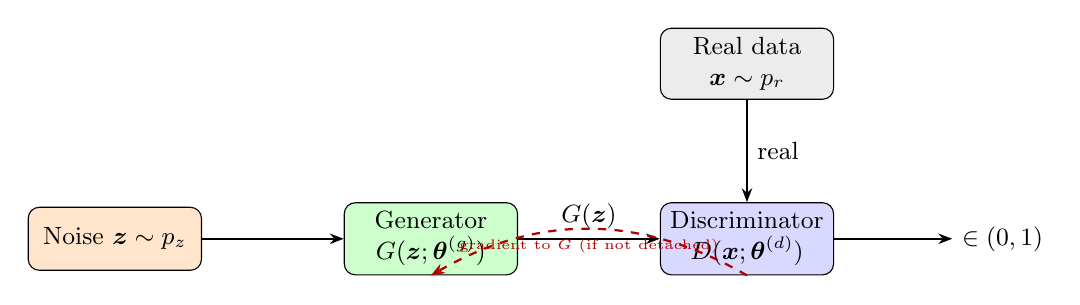
\begin{tikzpicture}[
      node distance=1.3cm and 1.8cm,
      box/.style={draw, rounded corners=4pt, minimum width=2.2cm,
                  minimum height=0.8cm, align=center, font=\small},
      arrow/.style={-{Stealth[length=5pt]}, thick}
    ]
    \node[box, fill=orange!20]  (noise)  {Noise $\bz\sim\pz$};
    \node[box, fill=green!20,   right=of noise] (G) {Generator\\$G(\bz;\btheta^{(g)})$};
    \node[box, fill=blue!15,    right=of G]     (D) {Discriminator\\$D(\bx;\btheta^{(d)})$};
    \node[box, fill=gray!15,    above=of D]     (real) {Real data\\$\bx\sim\pr$};
    \node[right=1.5cm of D, font=\small] (out) {$\in(0,1)$};

    \draw[arrow] (noise) -- (G) node[midway,above,font=\tiny] {};
    \draw[arrow] (G)     -- (D) node[midway,above,font=\small] {$G(\bz)$};
    \draw[arrow] (real)  -- (D) node[midway,right,font=\small] {real};
    \draw[arrow] (D)     -- (out);

    % Gradient arrows back
    \draw[arrow,dashed,red!70!black,bend right=30]
      (D.south) to node[below,font=\tiny,red!70!black]
      {gradient to $G$ (if not detached)} (G.south);
  \end{tikzpicture}
  \end{center}

  \medskip
  \begin{itemize}
    \item $G$ maps $\bz\in\R^k\to\R^d$ (noise $\to$ data space)
    \item $D$ maps $\bx\in\R^d\to(0,1)$ (image $\to$ probability)
    \item Training alternates: freeze $G$ and update $D$; freeze $D$ and update $G$
  \end{itemize}
\end{frame}

\begin{frame}{Learning Paradigms and Applications}
  \begin{columns}[T]
    \column{0.50\textwidth}
      \textbf{Three learning settings:}
      \begin{enumerate}
        \item \textbf{Unsupervised} — no labels; $G$ learns the full data manifold
        \item \textbf{Supervised} — conditional GAN conditions $G$ on class label
        \item \textbf{Semi-supervised} — $D$ doubles as a feature extractor
      \end{enumerate}

    \column{0.47\textwidth}
      \textbf{Applications:}
      \begin{itemize}
        \item Image synthesis / super-resolution
        \item Text-to-image translation
        \item Video prediction
        \item Data augmentation for rare events
        \item Anomaly detection
        \item Scientific simulation:\\
              particle physics, drug discovery,\\
              climate modelling
      \end{itemize}
  \end{columns}
\end{frame}

%% ═══════════════════════════════════════════════════════════
\section{Mathematical Formulation}
%% ═══════════════════════════════════════════════════════════

\begin{frame}{Notation and Probability Spaces}
  \begin{center}
  \renewcommand{\arraystretch}{1.25}
  \begin{tabular}{ll}
    \toprule
    Symbol & Meaning\\
    \midrule
    $\pr(\bx)$ & Real data distribution (unknown; represented by training set)\\
    $\pz(\bz)$ & Latent noise prior, e.g.\ $\mathcal{N}(\mathbf{0},I)$\\
    $G(\bz;\btheta^{(g)})$ & Generator: differentiable map $\R^k\to\R^d$\\
    $\pg$ & Generator distribution = push-forward of $\pz$ through $G$\\
    $D(\bx;\btheta^{(d)})\in(0,1)$ & Discriminator: $\Pr(\bx\text{ is real})$\\
    \bottomrule
  \end{tabular}
  \end{center}

  \medskip
  \textbf{Implicit distribution.} For invertible $G$ the change-of-variables gives:
  \[
    \pg(\bx) = \pz\!\left(G^{-1}(\bx)\right)\,
    \left|\det\frac{\partial G^{-1}}{\partial\bx}\right|.
  \]
  In practice $G$ is not invertible; $\pg$ is an \emph{implicit} distribution
  accessed only through sampling.
\end{frame}

\begin{frame}{The Minimax Objective}
  \begin{block}{Value function (Goodfellow et al., 2014)}
    \[
      \boxed{
        \min_{G}\;\max_{D}\;V(G,D)
        = \underbrace{\E_{\bx\sim\pr}[\log D(\bx)]}_{\text{$D$ correct on real}}
        + \underbrace{\E_{\bz\sim\pz}[\log(1-D(G(\bz)))]}_{\text{$D$ correct on fake}}
      }
    \]
  \end{block}

  \medskip
  \begin{columns}[T]
    \column{0.48\textwidth}
      \textbf{Discriminator (maximise $V$):}
      \begin{itemize}
        \item $D(\bx)\to 1$ on real data
        \item $D(G(\bz))\to 0$ on generated data
      \end{itemize}
    \column{0.48\textwidth}
      \textbf{Generator (minimise $V$):}
      \begin{itemize}
        \item $D(G(\bz))\to 1$ (fool $D$)
        \item $\E_{\pr}[\log D(\bx)]$ is constant w.r.t.\ $G$,
              so $G$ minimises $\E[\log(1-D(G(\bz)))]$
      \end{itemize}
  \end{columns}
\end{frame}

\begin{frame}{Non-Saturating Generator Loss}
  \begin{columns}[T]
    \column{0.52\textwidth}
      \textbf{Problem with the original objective.}
      Early in training $D$ is strong, so $D(G(\bz))\approx 0$:
      \[
        \frac{\partial}{\partial\btheta^{(g)}}\log(1-D(G(\bz)))
        \approx \frac{\partial}{\partial\btheta^{(g)}}\log 1 = 0.
      \]
      The gradient \emph{vanishes} before $G$ has learned anything.

    \column{0.45\textwidth}
      \begin{alertblock}{Fix: non-saturating loss}
        Instead of minimising $\log(1-D(G(\bz)))$,\\
        maximise $\log D(G(\bz))$:
        \[
          \mathcal{L}_G^{\text{non-sat}}
          = -\E_{\bz\sim\pz}[\log D(G(\bz))].
        \]
        Same Nash equilibrium; stronger gradient when $D(G(\bz))\approx 0$.
      \end{alertblock}
  \end{columns}

  \medskip
  \begin{center}
  \renewcommand{\arraystretch}{1.2}
  \begin{tabular}{lcc}
    \toprule
    Loss form & Value at $D(G(\bz))=\varepsilon\approx0$
              & $|\text{gradient}|$\\
    \midrule
    $\log(1-\varepsilon)$ & $\approx-\varepsilon$ & $\approx 1$ (small)\\
    $-\log\varepsilon$    & $+\infty$             & $1/\varepsilon\to\infty$ (large)\\
    \bottomrule
  \end{tabular}
  \end{center}
\end{frame}

\begin{frame}{The Alternating Gradient Algorithm}
  \begin{block}{One training iteration}
    \begin{enumerate}
      \setlength\itemsep{4pt}
      \item \textbf{Freeze $G$}; gradient \textbf{ascent} on $D$:
            \[
              \btheta^{(d)} \leftarrow \btheta^{(d)}
              + \eta\,\nabla_{\btheta^{(d)}}V(G,D).
            \]

      \item \textbf{Freeze $D$}; gradient \textbf{descent} on $G$:
            \[
              \btheta^{(g)} \leftarrow \btheta^{(g)}
              - \eta\,\nabla_{\btheta^{(g)}}\mathcal{L}_G.
            \]
    \end{enumerate}
  \end{block}

  \medskip
  \begin{itemize}
    \item One $D$ step per $G$ step in practice ($k=1$).
    \item Fake images are \textbf{detached} from the computation graph during
          the $D$ step to prevent spurious gradients flowing into $G$.
    \item Both networks update simultaneously — this does \emph{not} guarantee
          convergence (see Section~\ref{sec:challenges}).
  \end{itemize}
\end{frame}

%% ═══════════════════════════════════════════════════════════
\section{Optimal Discriminator and JS Divergence}
%% ═══════════════════════════════════════════════════════════

\begin{frame}{Deriving the Optimal Discriminator}
\small
  Fix $G$ (hence fix $\pg$). Write $V$ as an integral:
  \[
    V(G,D) = \int_{\bx}
    \bigl[\pr(\bx)\log D(\bx) + \pg(\bx)\log(1-D(\bx))\bigr]\,d\bx.
  \]

  \smallskip
  For each $\bx$ independently, maximise the integrand
  $f(t)=A\log t+B\log(1-t)$, $A=\pr(\bx)$, $B=\pg(\bx)$, $t=D(\bx)\in(0,1)$:
  \[
    f'(t) = \frac{A}{t} - \frac{B}{1-t}
    = \frac{A-(A+B)t}{t(1-t)} = 0
    \;\Longrightarrow\; t^* = \frac{A}{A+B}.
  \]

  Check: $f''(t^*) = -A/(t^*)^2 - B/(1-t^*)^2 < 0$ \; $\checkmark$ (maximum).

  \begin{block}{Optimal discriminator}
    \[
      \boxed{D^*(\bx) = \frac{\pr(\bx)}{\pr(\bx)+\pg(\bx)}.}
    \]
    This is the \textbf{Bayes-optimal classifier} for the two-class problem
    \{real, fake\} under equal class priors.
  \end{block}
\end{frame}

\begin{frame}{Nash Equilibrium and Loss at the Optimum}
  \begin{columns}[T]
    \column{0.50\textwidth}
      \textbf{Nash equilibrium.}
      At $\pg=\pr$:
      \[
        D^*(\bx) = \frac{\pr(\bx)}{\pr(\bx)+\pr(\bx)} = \frac{1}{2}.
      \]
      The discriminator cannot distinguish real from fake —
      it is reduced to random guessing.

      \medskip
      \textbf{Loss at the equilibrium.}
      Substituting $D^*=1/2$:
      \begin{align*}
        V(G^*,D^*)
        &= \log\!\tfrac{1}{2}\int\pr\,d\bx
         + \log\!\tfrac{1}{2}\int\pr\,d\bx\\
        &= -2\log 2 \approx -1.386.
      \end{align*}

    \column{0.47\textwidth}
      \begin{alertblock}{Convergence indicator}
        In practice, monitor $D(\bx)$ and $D(G(\bz))$ during training.
        Both should converge to $0.5$ at equilibrium.
        If $D(G(\bz))\ll 0.5$, the generator is losing.
        If $D(\bx)\ll 0.5$, the discriminator is failing.
      \end{alertblock}
  \end{columns}
\end{frame}

\begin{frame}{KL and JS Divergences}
  \textbf{Kullback-Leibler divergence:}
  \[
    \KL(p\|q) = \int p(\bx)\log\frac{p(\bx)}{q(\bx)}\,d\bx
    \;\ge 0,
  \]
  with equality iff $p=q$ a.e.\ (Gibbs' inequality).
  Note: $\KL(p\|q)\ne\KL(q\|p)$ in general.

  \smallskip
  \textbf{Jensen-Shannon divergence} (symmetric, bounded):
  \[
    \JS(p\|q)
    = \frac{1}{2}\KL\!\left(p\,\Big\|\,\frac{p+q}{2}\right)
    + \frac{1}{2}\KL\!\left(q\,\Big\|\,\frac{p+q}{2}\right).
  \]

  \begin{block}{Properties of $\JS$}
    \begin{itemize}
      \item Symmetric: $\JS(p\|q)=\JS(q\|p)$
      \item Non-negative: $\JS(p\|q)\ge 0$, with equality iff $p=q$
      \item Bounded: $\JS(p\|q)\in[0,\log 2]$ for any $p,q$
      \item Related to total variation: $\JS(p\|q)\le\log 2\cdot\mathrm{TV}(p,q)$
    \end{itemize}
  \end{block}
\end{frame}

\begin{frame}{GAN Loss $=$ Jensen-Shannon Divergence}
  Expanding $\JS(\pr\|\pg)$ and simplifying:
  \begin{align*}
    \JS(\pr\|\pg)
    &= \frac{1}{2}\KL\!\left(\pr\,\Big\|\,\frac{\pr+\pg}{2}\right)
     + \frac{1}{2}\KL\!\left(\pg\,\Big\|\,\frac{\pr+\pg}{2}\right)\\
    &= \frac{1}{2}\!\left(\log 2
       + \int\pr\log\frac{\pr}{\pr+\pg}\,d\bx\right)
     + \frac{1}{2}\!\left(\log 2
       + \int\pg\log\frac{\pg}{\pr+\pg}\,d\bx\right).
  \end{align*}

  Recognising $V(G,D^*)$ in the integrals:

  \begin{block}{Main theorem (Goodfellow et al.\ 2014)}
    \[
      \boxed{V(G,D^*) = 2\,\JS(\pr\|\pg) - 2\log 2.}
    \]
    \textbf{Conclusion.} The GAN minimax objective is equivalent to minimising the
    Jensen-Shannon divergence between $\pr$ and $\pg$.
    The global minimum $-2\log 2$ is achieved when $\pg=\pr$.
  \end{block}
\end{frame}

%% ═══════════════════════════════════════════════════════════
\section{Loss Functions in Practice}
%% ═══════════════════════════════════════════════════════════

\begin{frame}{Binary Cross-Entropy Losses}
\small
  \textbf{Discriminator loss} (real label $=s$, fake label $=0$):
  \[
    \mathcal{L}_D
    = -\frac{1}{N}\sum_{i=1}^N \log D(\bx_i)
      -\frac{1}{M}\sum_{j=1}^M \log\bigl(1-D(G(\bz_j))\bigr).
  \]
  \textbf{Generator loss} (non-saturating):
  \[
    \mathcal{L}_G
    = -\frac{1}{M}\sum_{j=1}^M \log D(G(\bz_j)).
  \]
  \begin{block}{One-sided label smoothing ($s=0.9$)}
    Replace real target $1$ with $s<1$. The optimal discriminator becomes
    $D^*_s(\bx) = s\cdot\pr(\bx)/(\pr(\bx)+\pg(\bx))$,
    preventing overconfidence and keeping gradients to $G$ alive.
  \end{block}
\end{frame}

\begin{frame}{Wasserstein Distance (WGAN)}
  \begin{columns}[T]
    \column{0.52\textwidth}
      \small
      \textbf{Problem with JS divergence.}
      When $\pr$ and $\pg$ have non-overlapping supports
      (common early in training): $\JS(\pr\|\pg)=\log 2$ constantly,
      giving zero gradient everywhere.

      \smallskip
      \textbf{Wasserstein-1 distance} (\emph{Earth-mover}):
      \begin{align*}
        W(\pr,\pg) &= \inf_{\gamma\in\Pi(\pr,\pg)}\,
          \E_{(\bx,\mathbf{y})\sim\gamma}\|\bx-\mathbf{y}\|
      \end{align*}
      $\Pi(\pr,\pg)$: all couplings with marginals $\pr$, $\pg$.

    \column{0.43\textwidth}
      \begin{block}{Kantorovich-Rubinstein duality}
        \[
          W(\pr,\pg) = \sup_{\|f\|_L\le 1}
          \bigl(\E_{\pr}[f] - \E_{\pg}[f]\bigr).
        \]
        Sup.\ over all 1-Lipschitz functions $f$.
      \end{block}
      \begin{alertblock}{Advantage}
        $W$ gives meaningful gradients
        even when $\pr\cap\pg=\emptyset$.
        Training is more stable.
      \end{alertblock}
  \end{columns}
\end{frame}

\begin{frame}{WGAN: Gradient Penalty}
  \textbf{WGAN critic.} Replace $D$ with a critic $f_w$ (no sigmoid):
  \[
    \mathcal{L}_{\mathrm{critic}}
    = \E_{\pg}[f_w(\bx)] - \E_{\pr}[f_w(\bx)]
    + \lambda\,\mathcal{L}_{\mathrm{GP}}.
  \]

  \textbf{Gradient penalty} (Gulrajani et al., 2017):
  \[
    \mathcal{L}_{\mathrm{GP}}
    = \E_{\hat{\bx}}\!\Bigl[
        \bigl(\|\nabla_{\hat{\bx}} f_w(\hat{\bx})\|_2 - 1\bigr)^2
      \Bigr],
  \]
  where $\hat{\bx} = \epsilon\bx + (1-\epsilon)G(\bz)$, $\epsilon\sim U[0,1]$
  (uniform on straight lines between real and fake points).

  \medskip
  \begin{itemize}
    \item Enforces the 1-Lipschitz constraint via soft penalisation.
    \item More stable than weight clipping (original WGAN).
    \item $\lambda=10$ is a standard choice.
  \end{itemize}
\end{frame}

%% ═══════════════════════════════════════════════════════════
\section{Training Challenges}
%% ═══════════════════════════════════════════════════════════

\begin{frame}{Vanishing Gradient}
  \textbf{When does it occur?}
  When $D$ is perfect early in training:
  $D(\bx)=1\;\forall\bx\sim\pr$ and $D(G(\bz))=0\;\forall\bz\sim\pz$.

  \medskip
  \textbf{Original $G$ gradient:}
  \[
    \nabla_{\btheta^{(g)}}\,\E[\log(1-D(G(\bz)))]
    \approx \nabla_{\btheta^{(g)}}\,\E[\log 1] = \mathbf{0}.
  \]
  No information flows to $G$.

  \medskip
  \textbf{Non-saturating loss $-\log D(G(\bz))$:}
  \[
    \nabla_{\btheta^{(g)}}\bigl(-\log D(G(\bz))\bigr)
    = -\frac{1}{D(G(\bz))}\nabla_{\btheta^{(g)}}D(G(\bz)).
  \]
  When $D(G(\bz))\approx 0$, the factor $1/D(G(\bz))\to\infty$ amplifies the gradient
  — learning continues.
\end{frame}

\begin{frame}{Mode Collapse}
  \begin{columns}[T]
    \column{0.52\textwidth}
      \textbf{Definition.} The generator maps many different noise vectors
      $\bz$ to the \emph{same} (or very few) output(s):
      \[
        \mathrm{supp}(\pg) \ll \mathrm{supp}(\pr).
      \]
      The JS divergence can still be low on the covered modes,
      so the loss does not detect collapse.

      \medskip
      \textbf{Why it happens.} Given the current discriminator,
      $G$ finds a single ``safe'' output that fools $D$;
      $D$ then adapts, and $G$ shifts to another single output.
      The two networks chase each other indefinitely.

    \column{0.45\textwidth}
      \textbf{Mitigations:}
      \begin{itemize}
        \item \textbf{Minibatch discrimination}: $D$ sees statistics of a
              batch, not individual images — diversity is rewarded.
        \item \textbf{Unrolled GANs}: $G$ optimises against a future $D$,
              preventing short-sighted collapse.
        \item \textbf{Spectral normalisation}: stabilises $D$ by bounding
              its Lipschitz constant.
        \item \textbf{WGAN}: Wasserstein distance measures full distribution
              mismatch, not just modes.
      \end{itemize}
  \end{columns}
\end{frame}

\begin{frame}{Non-Convergence and the Game-Theoretic View}
  GAN training solves a \textbf{two-player non-cooperative game}:
  \[
    G^* = \argmin_G\,\argmax_D\;V(G,D).
  \]

  \medskip
  \textbf{Nash equilibrium} exists at $\pg=\pr$, $D^*\equiv\tfrac{1}{2}$, but:
  \begin{itemize}
    \item Simultaneous gradient updates do \emph{not} guarantee convergence
          to a Nash equilibrium.
    \item The loss landscape of each player changes at every step
          (non-stationary environment).
    \item If $\max_D V(G,D)$ is not convex in $\btheta^{(g)}$,
          global convergence fails even in theory.
  \end{itemize}

  \medskip
  \textbf{Practical stabilisation:}
  \begin{itemize}
    \item Lower $\beta_1$ in Adam (reduces momentum: $0.5$ instead of $0.9$)
    \item One-sided label smoothing
    \item Spectral normalisation of $D$'s weights
    \item Progressive growing (ProGAN), self-attention (SAGAN)
    \item Two-time-scale updates: different learning rates for $G$ and $D$
  \end{itemize}
\end{frame}

%% ═══════════════════════════════════════════════════════════
\section{Evaluating GANs}
%% ═══════════════════════════════════════════════════════════

\begin{frame}{Evaluation Metrics: Overview}
  Evaluating generative models is hard: there is no ground truth output to compare against.

  \medskip
  \begin{center}
  \renewcommand{\arraystretch}{1.25}
  \begin{tabular}{p{2.8cm}p{4.5cm}p{3.5cm}}
    \toprule
    \textbf{Metric} & \textbf{Measures} & \textbf{Limitation}\\
    \midrule
    Inception Score (IS) & Quality + diversity of generated images & Requires pretrained classifier\\
    FID & Distance between real/fake feature distributions & Sensitive to sample size\\
    MMD & Kernel-based distribution distance & Choice of kernel matters\\
    Precision/Recall & Coverage vs.\ fidelity separately & Requires feature extractor\\
    \bottomrule
  \end{tabular}
  \end{center}
\end{frame}

\begin{frame}{Maximum Mean Discrepancy (MMD)}
  \textbf{Definition in RKHS.}  Let $k:\R^d\times\R^d\to\R$ be a kernel.
  The \textbf{MMD} between distributions $p$, $q$ is:
  \[
    \mathrm{MMD}^2(p,q)
    = \E_{\bx,\bx'\sim p}[k(\bx,\bx')]
    - 2\,\E_{\bx\sim p,\,\mathbf{y}\sim q}[k(\bx,\mathbf{y})]
    + \E_{\mathbf{y},\mathbf{y}'\sim q}[k(\mathbf{y},\mathbf{y}')].
  \]

  With the Gaussian kernel $k(\bx,\mathbf{y})=\exp(-\|\bx-\mathbf{y}\|^2/2\sigma^2)$:
  $\mathrm{MMD}=0$ iff $p=q$ (characteristic kernel property).

  \begin{block}{Unbiased empirical estimator}
    Given $n$ real samples $\{\bx_i\}$ and $m$ fake samples $\{\mathbf{y}_j\}$:
    \[
      \widehat{\mathrm{MMD}}^2
      = \frac{1}{n(n-1)}\!\sum_{i\ne j}\!k(\bx_i,\bx_j)
      - \frac{2}{nm}\sum_{i,j}\!k(\bx_i,\mathbf{y}_j)
      + \frac{1}{m(m-1)}\!\sum_{i\ne j}\!k(\mathbf{y}_i,\mathbf{y}_j).
    \]
    Diagonal terms ($i=j$) excluded for unbiasedness.
  \end{block}
\end{frame}

\begin{frame}{Fr\'echet Inception Distance (FID)}
  \textbf{FID} is currently the most widely used GAN metric.

  \medskip
  \textbf{Procedure:}
  \begin{enumerate}
    \item Extract feature vectors from the \textbf{InceptionV3} penultimate layer
          for $n$ real images and $n$ generated images.
    \item Fit Gaussians: $\mathcal{N}(\mu_r, \Sigma_r)$ and $\mathcal{N}(\mu_g, \Sigma_g)$.
    \item Compute the \textbf{Fr\'echet distance}:
  \end{enumerate}
  \[
    \mathrm{FID}
    = \|\mu_r - \mu_g\|^2
      + \mathrm{Tr}\!\Bigl(
          \Sigma_r + \Sigma_g
          - 2(\Sigma_r\Sigma_g)^{1/2}
        \Bigr).
  \]

  \begin{itemize}
    \item Lower FID = better quality and diversity.
    \item State-of-the-art GANs achieve FID $<5$ on MNIST; $<10$ on CIFAR-10.
    \item Sensitive to sample size $n$ — use $\ge 10\,000$ samples.
  \end{itemize}
\end{frame}

%% ═══════════════════════════════════════════════════════════
\section{Architecture Design}
%% ═══════════════════════════════════════════════════════════

\begin{frame}{Generator Architecture for MNIST}
  \textbf{Fully-connected generator} (Goodfellow et al., 2014 style):

  \small
  \[
    \bz\!\in\!\R^{100}
    \xrightarrow{\text{Lin+BN+LReLU}}
    \R^{256}
    \xrightarrow{\text{Lin+BN+LReLU}}
    \R^{512}
    \xrightarrow{\text{Lin+BN+LReLU}}
    \R^{1024}
    \xrightarrow{\text{Lin+Tanh}}
    \R^{784}
  \]
  \normalsize

  \medskip
  \begin{columns}[T]
    \column{0.50\textwidth}
      \textbf{Design choices:}
      \begin{itemize}
        \item \textbf{BatchNorm} after each Linear layer:\\
              normalises activations, allows higher LR,\\
              stabilises gradient flow
        \item \textbf{LeakyReLU(0.2):} prevents dying ReLU;\\
              small gradient for negative inputs
        \item \textbf{Tanh} output: maps to $[-1,1]$, matching\\
              MNIST normalised to $[-1,1]$
        \item Weights: $\mathcal{N}(0,0.02^2)$ (DCGAN convention)
      \end{itemize}

    \column{0.47\textwidth}
      \textbf{Discriminator differences:}
      \begin{itemize}
        \item \textbf{No BatchNorm}: introduces minibatch\\
              dependencies, causes instability in $D$
        \item \textbf{Dropout(0.3)}: regularises, prevents\\
              $D$ from over-fitting on real data
        \item \textbf{Sigmoid} output: probability in $(0,1)$
        \item Input: flattened image $\in\R^{784}$
      \end{itemize}
  \end{columns}
\end{frame}

\begin{frame}{Latent Space Interpolation}
  A well-trained generator has a \textbf{smooth latent space}.
  Linear interpolation between two noise vectors:
  \[
    \bz(\alpha) = (1-\alpha)\,\bz_1 + \alpha\,\bz_2,
    \quad \alpha\in[0,1]
  \]
  should yield a smooth visual transition between the corresponding images.

  \medskip
  \begin{itemize}
    \item \textbf{Smooth transitions}: generator has learned a good manifold.
    \item \textbf{Abrupt jumps}: mode collapse or poor latent coverage.
    \item Provides a qualitative test of latent space geometry that FID cannot capture.
  \end{itemize}

  \begin{alertblock}{Spherical interpolation}
    On a high-dimensional sphere (approximately the case for $\bz\sim\mathcal{N}(0,I)$),
    \emph{spherical} interpolation
    $\bz(\alpha) = \tfrac{\sin((1-\alpha)\Omega)}{\sin\Omega}\bz_1
                 + \tfrac{\sin(\alpha\Omega)}{\sin\Omega}\bz_2$,
    $\cos\Omega=\hat{\bz}_1\cdot\hat{\bz}_2$,
    stays on the noise manifold and gives more natural transitions.
  \end{alertblock}
\end{frame}

%% ═══════════════════════════════════════════════════════════
\section{Extensions and Variants}
%% ═══════════════════════════════════════════════════════════

\begin{frame}{Conditional GAN (cGAN)}
  \begin{columns}[T]
    \column{0.52\textwidth}
      A \textbf{conditional GAN} (Mirza \& Osindero, 2014) conditions both
      $G$ and $D$ on auxiliary information $\mathbf{y}$ (class label, image, text):

      \begin{align*}
        \min_G\max_D\;V(G,D)
        &= \E[\log D(\bx|\mathbf{y})]\\
        &\quad+ \E[\log(1-D(G(\bz|\mathbf{y})))].
      \end{align*}

      For MNIST: $\mathbf{y}$ is the digit class (one-hot, $\R^{10}$).
      Concatenate $\mathbf{y}$ to both $G$'s input $\bz$ and $D$'s input $\bx$.

    \column{0.45\textwidth}
      \begin{block}{cGAN enables}
        \begin{itemize}
          \item Controlled generation: specify which digit to generate
          \item Image-to-image translation (pix2pix)
          \item Text-to-image synthesis
          \item Style transfer
        \end{itemize}
      \end{block}
  \end{columns}
\end{frame}

\begin{frame}{Deep Convolutional GAN (DCGAN)}
  Radford, Metz, Chintala (ICLR 2016) replaced fully-connected layers
  with \textbf{strided convolutions}:

  \medskip
  \begin{itemize}
    \item \textbf{Generator}: fractionally strided convolutions (transposed conv)
          to upsample from $\bz\in\R^{100}$ to full-resolution image.
    \item \textbf{Discriminator}: strided convolutions to downsample.
    \item BatchNorm in $G$ (all layers except output); BatchNorm in $D$ (except input).
    \item ReLU in $G$; LeakyReLU in $D$.
    \item No pooling layers; no fully-connected layers (except for $\bz$).
  \end{itemize}

  \medskip
  \begin{alertblock}{Key advance}
    DCGAN produced the first visually convincing high-resolution GAN outputs
    and established the architectural conventions still used today.
    The DCGAN paper's guidelines (no BN in $D$ input layer, LReLU slope 0.2,
    Adam with $\beta_1=0.5$) remain standard practice.
  \end{alertblock}
\end{frame}

\begin{frame}{Comparison of GAN Variants}
  \begin{center}
  \small
  \renewcommand{\arraystretch}{1.2}
  \begin{tabular}{p{2.0cm}p{2.8cm}p{2.3cm}p{2.6cm}}
    \toprule
    \textbf{Variant} & \textbf{Key change} & \textbf{Loss} & \textbf{Advantage}\\
    \midrule
    Vanilla GAN & FC networks   & JS div.       & Simple\\
    DCGAN       & Conv.\ nets   & JS div.       & Better images\\
    WGAN        & Wt.\ clipping & Wasserstein   & More stable\\
    WGAN-GP     & Grad.\ penalty& Wasser.+GP    & No clipping\\
    cGAN        & Conditioning  & JS or W       & Controlled\\
    StyleGAN    & Style-based   & W             & SOTA\\
    \bottomrule
  \end{tabular}
  \end{center}
\end{frame}

%% ═══════════════════════════════════════════════════════════

% GAN Summary and Exercises
\section{Summary and Exercises}
%% ═══════════════════════════════════════════════════════════

\begin{frame}{Key Equations: Summary}
  \footnotesize
  \begin{center}
  \renewcommand{\arraystretch}{1.15}
  \begin{tabular}{ll}
    \toprule
    \textbf{Concept} & \textbf{Formula}\\
    \midrule
    Minimax objective
      & $\min_G\max_D\;\E_{\pr}[\log D(\bx)]+\E_{\pz}[\log(1-D(G(\bz)))]$\\[2pt]
    Optimal discriminator
      & $D^*(\bx) = \pr(\bx)/(\pr(\bx)+\pg(\bx))$\\[2pt]
    Nash equilibrium
      & $\pg=\pr$,\quad$D^*\equiv 1/2$\\[2pt]
    Loss at equilibrium
      & $V(G^*,D^*)=-2\log 2$\\[2pt]
    GAN loss = JS div.
      & $V(G,D^*)=2\JS(\pr\|\pg)-2\log 2$\\[2pt]
    Non-sat.\ generator
      & $\mathcal{L}_G=-\E_{\pz}[\log D(G(\bz))]$\\[2pt]
    Discriminator loss
      & $\mathcal{L}_D=-\E_{\pr}[\log D(\bx)]-\E_{\pz}[\log(1-D(G(\bz)))]$\\[2pt]
    Wasserstein distance
      & $W(\pr,\pg)=\sup_{\|f\|_L\le1}(\E_{\pr}[f]-\E_{\pg}[f])$\\[2pt]
    Gradient penalty
      & $\lambda\,\E[(\|\nabla f_w(\hat{\bx})\|_2-1)^2]$\\[2pt]
    MMD
      & $\sqrt{\E_{p\times p}[k]-2\E_{p\times q}[k]+\E_{q\times q}[k]}$\\[2pt]
    FID
      & $\|\mu_r-\mu_g\|^2+\mathrm{Tr}(\Sigma_r+\Sigma_g-2(\Sigma_r\Sigma_g)^{1/2})$\\
    \bottomrule
  \end{tabular}
  \end{center}
\end{frame}

\begin{frame}{Exercises}
  \begin{enumerate}
    \setlength\itemsep{5pt}
    \item \textbf{Optimal discriminator.}
          Derive $D^*(\bx)=\pr/(\pr+\pg)$ by differentiating
          $f(t)=A\log t+B\log(1-t)$ and verify it is a maximum, not a minimum.

    \item \textbf{JS divergence bounds.}
          Prove $\JS(p\|q)\in[0,\log 2]$ for any two distributions and
          find the conditions for equality on each side.

    \item \textbf{Vanishing gradient.}
          At $D(G(\bz))=\varepsilon\ll 1$, compute
          $|\nabla_{\btheta^{(g)}}\mathcal{L}_G^{\text{orig}}|$ and
          $|\nabla_{\btheta^{(g)}}\mathcal{L}_G^{\text{non-sat}}|$
          and compare their magnitudes as $\varepsilon\to 0$.

    \item \textbf{Label smoothing.}
          Derive the optimal discriminator $D^*_s(\bx)$ when real targets
          are smoothed to $s\in(0,1)$ instead of $1$.
          Show it converges to $D^*$ as $s\to 1$.

    \item \textbf{Wasserstein distance.}
          Compute $W(\mathcal{N}(0,1),\mathcal{N}(\mu,1))$ analytically
          and verify that $W\to 0$ as $\mu\to 0$, unlike $\JS$ when the
          two Gaussians have non-overlapping support.

    \item \textbf{Conditional GAN.}
          Extend the minimax objective to the conditional setting.
          What changes in the derivation of $D^*(\bx|\mathbf{y})$?
  \end{enumerate}
\end{frame}

% =============================================================================
\section{Comparing Generative Models: VAEs, Diffusion, and GANs}
% =============================================================================

\begin{frame}{Three Families: A Unified Mathematical View}
\small
All three learn $p_{\btheta}(\bx)$ but with different objectives and inductive biases.

\begin{center}
\renewcommand{\arraystretch}{1.15}
\begin{tabular}{llll}
\toprule
\textbf{Criterion}  & \textbf{VAE}   & \textbf{Diffusion} & \textbf{GAN}\\
\midrule
Objective      & ELBO           & ELBO ($T$ terms)   & Minimax / JS\\
Likelihood     & $\checkmark$   & $\checkmark$       & $\times$\\
Latent space   & Compact $\bh$  & Full-dim $\bx_t$   & Noise $\bz$\\
Encoder        & Learned        & Fixed schedule     & None\\
Sampling cost  & 1 decoder pass & $T$ steps          & 1 pass\\
Stability      & High           & High               & Low--Moderate\\
Sample quality & Moderate       & State of the art   & High (sharp)\\
Mode coverage  & Good           & Excellent          & Partial\\
Anomaly detect.& $\checkmark$   & $\checkmark$       & $\times$\\
\bottomrule
\end{tabular}
\end{center}
\end{frame}

\begin{frame}{Why VAEs Produce Blurry Samples}

\textbf{Mathematical reason.}
The VAE decoder minimises:
\[
  -\E_{q_{\bphi}(\bh|\bx)}\!\bigl[\log p_{\btheta}(\bx|\bh)\bigr]
  \;\propto\;
  \E_{q_{\bphi}}\!\bigl[\|\bx - \hat\bx_{\btheta}(\bh)\|^2\bigr].
\]
Because the posterior $q_{\bphi}(\bh|\bx)$ has nonzero variance,
the decoder learns the \textbf{posterior mean over all likely completions},
which is a blur over the data manifold.

\medskip
\textbf{Contrast with the other two models:}

\begin{columns}[T]
\column{0.48\textwidth}
\begin{block}{Diffusion avoids blurring by}
predicting only the \emph{noise added at one step} $t$, not the full image.
Each reverse step makes a small, committed correction.
The iterative nature removes the need to average over the full
distribution of plausible outputs.
\end{block}

\column{0.48\textwidth}
\begin{block}{GANs avoid blurring by}
replacing the fixed $\ell_2$ loss with an \emph{adaptive, learned}
discriminator loss. The discriminator penalises blurriness and any
systematic deviation from real data, providing a richer training signal
than any fixed pixel-wise objective.
\end{block}
\end{columns}
\end{frame}

\begin{frame}{The Likelihood Problem in GANs}

\textbf{A fundamental asymmetry.}
VAEs and diffusion models optimise a lower bound on $\log p(\bx)$,
so they can both \emph{generate} and \emph{evaluate} density.
GANs have \textbf{no access to $p_g(\bx)$}.

\medskip
\textbf{Consequences of no likelihood:}
\begin{itemize}
  \item Cannot compute log-likelihood scores for anomaly detection.
  \item Cannot evaluate model fit on held-out data in a principled way.
  \item Evaluation requires proxy metrics (FID, IS, MMD) rather than
        test-set log-likelihood.
  \item Cannot be embedded as a prior in a Bayesian framework without
        approximation.
\end{itemize}

\medskip
\textbf{Why this is a price worth paying (sometimes).}
The discriminator provides a \emph{perceptual} loss that no fixed
$p_{\btheta}$ objective can replicate: it adapts to what ``looks real''
to a neural network, capturing texture, sharpness, and high-frequency detail
that $\ell_2$ and even ELBO objectives systematically underweight.
\end{frame}

\begin{frame}{Training Stability: A Comparison}
\footnotesize
\begin{columns}[T]
\column{0.33\textwidth}
\begin{block}{VAE — Stable}
ELBO is a well-defined scalar.
Both networks trained with standard SGD.
KL prevents collapse when weighted correctly.
Main challenge: choosing $\beta$ for $\beta$-VAE.
\end{block}

\column{0.33\textwidth}
\begin{block}{Diffusion — Stable}
MSE on noise prediction is smooth.
No adversarial dynamics.
Low MC gradient variance ($\bx_t$ sampled in one step).
Main challenge: noise schedule design.
\end{block}

\column{0.32\textwidth}
\begin{block}{GAN — Unstable}
Non-stationary minimax landscape.
No Nash convergence guarantee.
$V(G,D)$ is concave-convex; simultaneous gradient ascent-descent
diverges even for bilinear games.
Requires WGAN-GP, spectral norm, label smoothing.
\end{block}
\end{columns}

\smallskip
\begin{alertblock}{Key insight}
GAN instability is \emph{fundamental}: the minimax saddle structure prevents
convergence guarantees that both VAE and DDPM enjoy.
\end{alertblock}
\end{frame}

\begin{frame}{Mode Collapse vs.\ Posterior Averaging: Two Failure Modes}

The two pathological failure modes of generative models lie at opposite ends:

\medskip
\begin{columns}[T]
\column{0.48\textwidth}
\begin{block}{Posterior averaging (VAE)}
\textbf{Too much spread.}
The decoder must explain all data through a single mean.
Result: generated images are averages over the data manifold — blurry.
The model \emph{covers} all modes but fails to commit to any one of them.
\[
  \hat\bx = \E_{q_{\bphi}(\bh|\bx)}[\hat\bx_{\btheta}(\bh)]
  \;\approx\;\text{mean of modes}
\]
\end{block}

\column{0.48\textwidth}
\begin{block}{Mode collapse (GAN)}
\textbf{Too little spread.}
The generator finds a single safe output that fools $D$
and ignores the rest of $p_r$.
Result: sharp images but only from a few modes.
$\mathrm{supp}(\pg)\ll\mathrm{supp}(\pr)$.
\[
  G(\bz) \approx \bx^*\;\forall\bz
  \;\Rightarrow\;
  \JS(\pr\|\pg)\approx\log 2\;\text{(flat)}
\]
\end{block}
\end{columns}

\medskip
\textbf{Diffusion avoids both:}
the fixed encoder $q(\bx_t|\bx_{t-1})$ prevents collapse
(no network can ``cheat'' the noise schedule),
and the iterative denoising avoids averaging because each step commits
to only a small noise correction rather than a full image prediction.
\end{frame}

\begin{frame}{Detailed Pros and Cons: VAEs}
\begin{columns}[T]
\column{0.5\textwidth}
\textcolor{green!60!black}{\textbf{Pros}}
\begin{itemize}\footnotesize\setlength\itemsep{2pt}
  \item \textbf{Likelihood bound}: ELBO usable for anomaly detection.
  \item \textbf{Compact latent}: $\bh$ supports interpolation, clustering,
        disentanglement, property prediction.
  \item \textbf{Fast generation}: single decoder pass.
  \item \textbf{Stable training}: well-defined ELBO, no adversary.
  \item \textbf{Flexible}: $\beta$-VAE for disentanglement;
        hierarchical VAEs for expressivity.
  \item \textbf{Scientific use}: ideal for molecules, spectra, simulations.
\end{itemize}

\column{0.48\textwidth}
\textcolor{red!60!black}{\textbf{Cons}}
\begin{itemize}\footnotesize\setlength\itemsep{2pt}
  \item \textbf{Blurry samples}: posterior averaging is fundamental,
        not a capacity issue.
  \item \textbf{Posterior collapse}: decoder ignores $\bh$;
        KL$\to 0$, latent useless.
  \item \textbf{ELBO gap}: $\log p(\bx)=\mathrm{ELBO}+
        \DKL(q_{\bphi}\|p(\bh|\bx))>\mathrm{ELBO}$.
  \item \textbf{Mean-field}: factorised Gaussian misses correlated posteriors.
  \item \textbf{Fixed-dim bottleneck}: wrong $d_h$ hurts quality.
\end{itemize}
\end{columns}
\end{frame}

\begin{frame}{Detailed Pros and Cons: Diffusion Models}
\begin{columns}[T]
\column{0.5\textwidth}
\textcolor{green!60!black}{\textbf{Pros}}
\begin{itemize}\footnotesize\setlength\itemsep{2pt}
  \item \textbf{Best sample quality}: sharp, diverse, no blurring.
  \item \textbf{Full coverage}: fixed forward process prevents mode collapse.
  \item \textbf{Stable training}: MSE on noise, no adversarial dynamics.
  \item \textbf{Likelihood bound}: ELBO $\to\log p(\bx)$ as $T\to\infty$.
  \item \textbf{Flexible conditioning}: text, class, depth via
        classifier-free guidance and cross-attention.
  \item \textbf{Rich theory}: SDE/score connection (Song et al.\ 2021).
\end{itemize}

\column{0.48\textwidth}
\textcolor{red!60!black}{\textbf{Cons}}
\begin{itemize}\footnotesize\setlength\itemsep{2pt}
  \item \textbf{Slow sampling}: $T\!=\!100$--$1000$ steps
        (DDIM/DPM-Solver: 10--50).
  \item \textbf{No compact latent}: full-dim $\bx_t$ precludes clustering
        or property prediction.
  \item \textbf{Compute-intensive}: large $T$, high-dim $\bx$ need
        significant GPU memory.
  \item \textbf{Poor for repr.\ learning}: no encoder for features.
  \item \textbf{Schedule-sensitive}: cosine preferred over linear
        at high resolution.
\end{itemize}
\end{columns}
\end{frame}

\begin{frame}{Detailed Pros and Cons: GANs}
\begin{columns}[T]
\column{0.5\textwidth}
\textcolor{green!60!black}{\textbf{Pros}}
\begin{itemize}\footnotesize\setlength\itemsep{2pt}
  \item \textbf{Sharpest samples}: adversarial loss catches blurriness
        that $\ell_2$/ELBO miss.
  \item \textbf{Fastest inference}: single generator pass.
  \item \textbf{Flexible loss}: works when likelihood is intractable.
  \item \textbf{Rich ecosystem}: cGAN, DCGAN, WGAN-GP, StyleGAN, pix2pix.
  \item \textbf{Image translation}: handles paired and unpaired transfer.
\end{itemize}

\column{0.48\textwidth}
\textcolor{red!60!black}{\textbf{Cons}}
\begin{itemize}\footnotesize\setlength\itemsep{2pt}
  \item \textbf{No likelihood}: no anomaly detection or density estimation.
  \item \textbf{Mode collapse}: $G$ covers only part of $p_r$;
        FID/IS may not detect it.
  \item \textbf{Instability}: non-stationary minimax; no convergence
        guarantee; hyperparameter-sensitive.
  \item \textbf{JS flatness}: $\JS\!=\!\log 2$ when supports don't overlap
        (WGAN fixes this).
  \item \textbf{Wasted discriminator}: $D$ discarded after training.
\end{itemize}
\end{columns}
\end{frame}

\begin{frame}{When to Use Each Model}
\footnotesize
\begin{center}
\renewcommand{\arraystretch}{1.0}
\begin{tabular}{p{3.8cm}p{2.1cm}p{3.8cm}}
\toprule
\textbf{Use case} & \textbf{Model} & \textbf{Reason}\\
\midrule
Image / audio / video synthesis & Diffusion & Best quality, no collapse\\
Text-to-image (Stable Diffusion) & LDM & VAE compression + diffusion\\
Image-to-image translation & GAN & Adversarial perceptual loss\\
Real-time generation & VAE or GAN & Single-pass inference\\
Anomaly detection & VAE or Diffusion & Likelihood bound available\\
Representation / clustering & VAE & Compact structured latent\\
Scientific data (molecules) & VAE & Low-dim latent for prediction\\
Data augmentation & GAN or Diffusion & Sharp, diverse samples\\
Inpainting / super-resolution & Diffusion & Score-based posterior\\
Very limited data & VAE & Stable; KL regularisation\\
\bottomrule
\end{tabular}
\end{center}
\end{frame}

\begin{frame}{Key Equations: Complete Summary Across All Three Models}
\footnotesize
\begin{center}
\renewcommand{\arraystretch}{1.15}
\begin{tabular}{p{3.2cm}p{4.2cm}p{4.2cm}}
\toprule
\textbf{Concept} & \textbf{VAE / Diffusion} & \textbf{GAN}\\
\midrule
Encoder &
  $q_{\bphi}(\bh|\bx)=\Norm(\bmu_{\bphi},\bsig^2_{\bphi}\mathbf{I})$\newline
  $q(\bx_t|\bx_{t-1})=\Norm(\sqrt{\alpha_t}\bx_{t-1},(1-\alpha_t)\mathbf{I})$ &
  None (implicit via $G$) \\[4pt]
Marginal / forward &
  $\bx_t=\sqrt{\bar\alpha_t}\bx_0+\sqrt{1-\bar\alpha_t}\beps$ &
  $\bx=G(\bz;\btheta^{(g)})$ \\[4pt]
Objective &
  $\ELBO = \E[\log p_{\btheta}(\bx|\bh)] - \DKL(q\|p)$ &
  $\min_G\max_D\,\E[\log D(\bx)]+\E[\log(1-D(G(\bz)))]$ \\[4pt]
Optimal solution &
  DDPM: $\bmu_{\btheta}=\frac{1}{\sqrt{\alpha_t}}(\bx_t-\frac{\beta_t}{\sqrt{1-\bar\alpha_t}}\beps_{\btheta})$ &
  $D^*(\bx)=\frac{\pr(\bx)}{\pr(\bx)+\pg(\bx)}$ \\[4pt]
Loss at equilibrium &
  VAE ELBO $\to\log p(\bx)$ &
  $V(G^*,D^*)=-2\log 2$ \\[4pt]
Divergence minimised &
  $\DKL(q\|p)$ at each level &
  $\JS(\pr\|\pg)$ \\[4pt]
Score connection &
  $\bm{s}_{\btheta}=-\beps_{\btheta}/\sqrt{1-\bar\alpha_t}$ &
  $D^*\to$ implicit score estimator \\[4pt]
Sampling &
  1 pass (VAE); $T$ steps (DDPM) &
  1 pass \\[4pt]
\bottomrule
\end{tabular}
\end{center}
\end{frame}

\begin{frame}{Exercises: Cross-Model Comparisons}
\begin{columns}[T]
\column{0.5\textwidth}
\begin{block}{Exercises 1--3}
\footnotesize
\begin{enumerate}
  \setlength\itemsep{4pt}
  \item \textbf{Common ELBO.}
        Show VAE (1 level) and DDPM ($T$ levels) are special cases of
        the MHVAE ELBO. Identify encoder, decoder, prior in each.

  \item \textbf{Blurriness from $\ell_2$.}
        For $p_r=\tfrac{1}{2}\delta(x\!-\!a)+\tfrac{1}{2}\delta(x\!-\!b)$,
        show the VAE decoder learns $\hat x=(a+b)/2$
        while a GAN can produce both modes.

  \item \textbf{Convergence.}
        State which property of the DDPM ELBO makes it amenable to SGD
        while the GAN minimax saddle is not.
\end{enumerate}
\end{block}

\column{0.5\textwidth}
\begin{block}{Exercises 4--6}
\footnotesize
\begin{enumerate}
  \setlength\itemsep{4pt}
  \setcounter{enumi}{3}
  \item \textbf{Wasserstein vs.\ JS.}
        Compute $\JS(\Norm(0,1)\|\Norm(\mu,1))$ and $W(\Norm(0,1),\Norm(\mu,1))$.
        Show $\JS$ saturates at $\log 2$ while $W=|\mu|$ grows.

  \item \textbf{Score matching bridge.}
        Using $\nabla_{\bx_t}\log q(\bx_t|\bx_0)=-\beps/\sqrt{1-\bar\alpha_t}$,
        show DDPM equals denoising score matching (Vincent 2011).

  \item \textbf{Latent Diffusion.}
        Express the LDM objective as a composition of VAE ELBO and DDPM ELBO.
        Identify which parameters are trained in each stage.
\end{enumerate}
\end{block}
\end{columns}
\end{frame}

\begin{frame}{References}
\begin{columns}[T]
\column{0.5\textwidth}
\textbf{Diffusion models}
\begin{enumerate}\footnotesize
  \setlength\itemsep{2pt}
  \item Kingma \& Welling, \emph{Auto-Encoding Variational Bayes},
        ICLR 2014. \href{https://arxiv.org/abs/1312.6114}{1312.6114}
  \item Ho, Jain \& Abbeel, \emph{DDPM},
        NeurIPS 2020. \href{https://arxiv.org/abs/2006.11239}{2006.11239}
  \item Song et al., \emph{Score-Based Generative Modeling through SDEs},
        ICLR 2021. \href{https://arxiv.org/abs/2011.13456}{2011.13456}
  \item Song, Meng \& Ermon, \emph{DDIM},
        ICLR 2021. \href{https://arxiv.org/abs/2010.02502}{2010.02502}
  \item Kingma et al., \emph{Variational Diffusion Models},
        NeurIPS 2021. \href{https://arxiv.org/abs/2107.00630}{2107.00630}
  \item Nichol \& Dhariwal, \emph{Improved DDPM},
        ICML 2021. \href{https://arxiv.org/abs/2102.09672}{2102.09672}
  \item Rombach et al., \emph{Latent Diffusion Models},
        CVPR 2022. \href{https://arxiv.org/abs/2112.10752}{2112.10752}
  \item Luo, \emph{Understanding Diffusion Models},
        2022. \href{https://arxiv.org/abs/2208.11970}{2208.11970}
\end{enumerate}

\column{0.48\textwidth}
\textbf{Generative Adversarial Networks}
\begin{enumerate}\footnotesize
  \setlength\itemsep{2pt}
  \item Goodfellow et al., \emph{Generative Adversarial Nets},
        NeurIPS 2014. \href{https://arxiv.org/abs/1406.2661}{1406.2661}
  \item Mirza \& Osindero, \emph{Conditional GAN},
        2014. \href{https://arxiv.org/abs/1411.1784}{1411.1784}
  \item Radford, Metz \& Chintala, \emph{DCGAN},
        ICLR 2016. \href{https://arxiv.org/abs/1511.06434}{1511.06434}
  \item Arjovsky, Chintala \& Bottou, \emph{WGAN},
        ICML 2017. \href{https://arxiv.org/abs/1701.07875}{1701.07875}
  \item Gulrajani et al., \emph{WGAN-GP},
        NeurIPS 2017. \href{https://arxiv.org/abs/1704.00028}{1704.00028}
  \item Heusel et al., \emph{FID},
        NeurIPS 2017. \href{https://arxiv.org/abs/1706.08500}{1706.08500}
  \item Goodfellow, Bengio \& Courville,
        \emph{Deep Learning}, MIT Press 2016, Ch.~20.
  \item Weng, \emph{From GAN to WGAN}, blog post, 2017.
\end{enumerate}
\end{columns}
\end{frame}
\end{document}
